%%
%% Copyright 2021 OXFORD UNIVERSITY PRESS
%%
%% This file is part of the 'ima-authoring-template Bundle'.
%% ---------------------------------------------
%%
%% It may be distributed under the conditions of the LaTeX Project Public
%% License, either version 1.2 of this license or (at your option) any
%% later version.  The latest version of this license is in
%%    http://www.latex-project.org/lppl.txt
%% and version 1.2 or later is part of all distributions of LaTeX
%% version 1999/12/01 or later.
%%
%% The list of all files belonging to the 'ima-authoring-template Bundle' is
%% given in the file `manifest.txt'.
%%
%% Template article for OXFORD UNIVERSITY PRESS's document class `ima-authoring-template'
%% with bibliographic references
%%

\documentclass[numbers,webpdf]{ima-authoring-template}%
%\documentclass[namedate,webpdf]{ima-authoring-template}

%\usepackage{showframe}

\graphicspath{{Fig/}}

% line numbers
%\usepackage[mathlines, switch]{lineno}
%\usepackage[right]{lineno}

\theoremstyle{thmstyletwo}%
\newtheorem{theorem}{Theorem}%  meant for continuous numbers
%%\newtheorem{theorem}{Theorem}[section]% meant for sectionwise numbers
%% optional argument [theorem] produces theorem numbering sequence instead of independent numbers for Proposition
\newtheorem{proposition}[theorem]{Proposition}%
%%\newtheorem{proposition}{Proposition}% to get separate numbers for theorem and proposition etc.

\newtheorem{example}{Example}%
\newtheorem{remark}{Remark}%
\newtheorem{lemma}{Lemma}%
\newtheorem{assumption}{Assumption}%
\newtheorem{definition}{Definition}

\numberwithin{equation}{section}

% added by user
\usepackage{xfrac} % to use \sfrac{}{}
\usepackage{physics} % to use \norm{}
\usepackage{amssymb} % to use \lesssim
\newcommand{\almosteverywhere}{\mathrm{a.e.}\;}
\DeclareMathOperator*{\esssup}{ess\,sup}
\DeclareMathOperator*{\essinf}{ess\,inf}
\usepackage{bm} %\mathbf{} does not work
\usepackage{upgreek}
\allowdisplaybreaks

\begin{document}

\DOI{DOI HERE}
\copyrightyear{2021}
\vol{00}
\pubyear{2021}
\access{Advance Access Publication Date: Day Month Year}
\appnotes{Paper}
\copyrightstatement{Published by Oxford University Press on behalf of the Institute of Mathematics and its Applications. All rights reserved.}
\firstpage{1}

%\subtitle{Subject Section}

\title[Numerical approximation of fractional diffusion equations on metric graphs]{Numerical approximation of fractional diffusion equations on metric graphs}

\author{David Bolin\ORCID{0000-0003-2361-5465}, Lenin Riera-Segura$^\dagger$\ORCID{0000-0002-4803-4918}, and Alexandre B. Simas\ORCID{0000-0003-2562-2829} \thanks{The authors are listed in alphabetical order.} \address{\orgdiv{Statistics Program, Computer, Electrical and Mathematical Sciences and Engineering (CEMSE) Division}, \orgname{King Abdullah University of Science and Technology (KAUST)}, \orgaddress{\postcode{23955-6900}, \state{Thuwal}, \country{Kingdom of Saudi Arabia}}}}

\authormark{David Bolin, Lenin Riera-Segura, and Alexandre B. Simas}

\corresp[$^\dagger$]{Corresponding author: \href{email:email-id.com}{leninrafael.rierasegura@kaust.edu.sa}}

\received{Date}{0}{Year}
\revised{Date}{0}{Year}
\accepted{Date}{0}{Year}

%\editor{Associate Editor: Name}

\abstract{We study fractional diffusion equations on compact metric graphs, where the nonlocal dynamics is governed by fractional powers of the shifted Kirchhoff–Laplacian. We establish fractional elliptic projection estimates and stability bounds relating continuous and discrete fractional operators, and derive error estimates for a fully discrete scheme combining backward Euler time-stepping with finite element discretization. To approximate the action of the fractional operator, we employ rational approximations, reducing the problem to a sequence of sparse elliptic solves for efficient implementation. We derive error estimates for the temporal, spatial, and rational discretizations, and confirm convergence through numerical experiments.}
\keywords{fractional Sobolev spaces; fractional Laplacian; shifted Kirchhoff--Laplacian; finite elements; analytic semigroup; rational approximation.}

% \boxedtext{
% \begin{itemize}
% \item Key boxed text here.
% \item Key boxed text here.
% \item Key boxed text here.
% \end{itemize}}

\maketitle

\section{Introduction}
\label{sec:introduction}
In recent years, there has been growing interest in dynamical processes on networks \cite{Cordoni2017Stochasticreactiondiffusion}, driven by applications ranging from disease spread \cite{Pastor2015Epidemicprocess} and information propagation in social networks \cite{Du2018PDE} to gas pipeline systems \cite{Herty2010Anewmodelforgasflow}, among others, where the underlying dynamics are often modeled by partial differential equations (PDEs) \cite{bottcher2024dynamicalprocessesmetricnetworks}. These include a broad range of physical models, such as Schrödinger, wave, and Klein--Gordon equations \cite{Dutykh2018Wave, Goloshchapova2021Anonlinear, Goodman2019NLSbifurcations, Goodman2025QGlAB}, as well as stochastic space--time models \cite{Cordoni2017Stochasticreactiondiffusion, Kovacs2021Stochastics}. A fundamental class of such dynamics is diffusion, which serves as a core model for the propagation of mass, energy, or information across networked systems \cite{Barrat2008Dynamicalprocess, Jivkov2014Anetworkmodel}. Parabolic PDEs, in particular, frequently arise in this setting as they effectively capture the temporal evolution of diffusive processes on networks. For instance, Weller \cite{kups73182} employed parabolic equations on metric graphs to simulate the distribution of tau proteins in the brain's structural network, offering insights into the progression of Alzheimer’s disease. See \cite[Chapter~11]{Danko2017Modelelements} and \cite{Pastor2015Epidemicprocess, Raj2012Anetworkdiffusionmodel} for additional examples of diffusion modeling on networks. 

Classical diffusion, however, may fail to capture the observed dynamics, especially when long-range interactions are present \cite{Daoud2025classp, Daoud2024Aclass}. This has led to increasing interest in fractional diffusion as a model for anomalous transport \cite{Vazquez2017Themathematical}. In space-fractional models, the standard spatial diffusion operator is replaced by a fractional counterpart, such as a fractional Laplacian, to incorporate nonlocal interactions. For further discussion of anomalous diffusion across different domains, see \cite{Henry2006Anomalous, Miller2006Onthecontrollability, Riascos2014Fractional, Somathilake2018Aspacefractional} and the references therein. On metric graphs, these models allow both anomalous transport and the underlying network topology to influence the evolution, with the fractional spatial operator governing the nonlocal dynamics.

To date, studies of fractional diffusion on metric graphs have primarily focused on time-fractional models \cite{Faheem2023Acollocation, Kumari2025Finite, Mehandiratta2021Optimalcontrol}. Existing works on space-fractional diffusion are comparatively few \cite{Leugering2023Optimalcontrol} and, together with the time-fractional studies, have been restricted to relatively simple graph topologies, such as star graphs. In this work, we consider space-fractional diffusion defined through the spectral powers of the shifted Kirchhoff--Laplacian on general compact metric graphs. Specifically, we analyze and numerically approximate solutions to equations of the form

\begin{equation}
\label{eq:maineq}
\left\{
\begin{aligned}
    \partial_t u(s,t) + (\kappa^2 - \Delta_\Gamma)^{\sfrac{\alpha}{2}} u(s,t) &= f(s,t), && \quad (s,t) \in \Gamma \times (0, T), \\
    u(s,0) &= u_0(s), && \quad s \in \Gamma.
\end{aligned}
\right.
\end{equation}
Here $\Gamma=(\mathcal{V},\mathcal{E})$ is a compact connected metric graph, $\kappa>0$, and $\alpha\in(0,2]$ is the spatial order of the diffusion operator. Further, $f:\Gamma\times(0,T)\to\mathbb{R}$ and $u_0:\Gamma\to\mathbb{R}$ are the prescribed source and initial condition, respectively. We write $L=\kappa^2-\Delta_\Gamma$, where $\Delta_\Gamma$ is the Kirchhoff--Laplacian. Its domain incorporates the vertex conditions
\begin{equation}
\label{eq:Kcond}
   \mathcal{K} =  \left\{\phi\in C(\Gamma)\cap \textstyle\bigoplus_{e\in\mathcal{E}} C^{1}(e)\;\middle|\; \forall v\in \mathcal{V}:\; \textstyle\sum_{s\in v}\partial \phi(s)=0 \right\},
\end{equation}
which express continuity and conservation of flux at each vertex. The vertex conditions are thus encoded in $L$ and in the fractional domains $\dot{H}^{s}(\Gamma)=D(L^{\sfrac{s}{2}})$. Details will be provided in later sections.

The numerical approximation of fractional diffusion has been studied through several approaches, depending on the definition of the fractional operator. On Euclidean domains, Glusa and Otárola \cite{Glusa2021errorestimates} considered the integral fractional Laplacian in an optimal control problem and derived error estimates for a scheme combining backward Euler time-stepping with piecewise linear finite elements. For spectral fractional powers, Bonito et al. \cite{Bonito2017Theapproximation} analyzed a finite element approximation of the parabolic solution operator and used contour quadrature for its numerical evaluation. Another approach uses an extension problem in a higher-dimensional domain \cite{Nochetto2016APDEapproach}. We refer to \cite{Bonito2018Numericalmethods} for a broader discussion of these formulations and their numerical approximation.

On metric graphs, Arioli and Benzi \cite{arioli2018finite} developed finite element methods for quantum graph problems. More recently, Bolin et al. \cite{bolin2023regularity} established regularity and numerical approximation results for fractional elliptic equations on compact metric graphs. Their characterization of fractional Sobolev spaces provides the functional framework for the present work, and their estimates for inverse fractional powers enter our spatial error analysis. Analyzing the evolution problem also requires control of how these approximation errors propagate through successive time steps and accumulate through the time-dependent source. We develop this analysis for a scheme combining backward Euler time-stepping, with step size $\tau$, and continuous, piecewise linear finite elements on conforming, quasi-uniform graph meshes of size $h$.

Our analytical contributions include approximation estimates in the spectral Sobolev spaces $\dot H^s(\Gamma)$. Lemma~\ref{lem:graph-fractional-fe-approx} establishes best-approximation bounds of order $h^{s-t}$ for $0\leq t\leq1$ and $t\leq s\leq2$, including the low-regularity range where nodal interpolation is not available. Proposition~\ref{proposition:with_elliptic_projection} then gives the estimate $\|\phi-G_{h,\alpha}\phi\|_{L_2(\Gamma)}\lesssim h^\alpha\|\phi\|_{\dot H^\alpha(\Gamma)}$ for the elliptic projection defined by the fractional energy form. This extends the second-order projection estimate in \cite[Proposition~6.2]{bolin2023regularity} to $0<\alpha\leq2$. In addition, Proposition~\ref{prop:controlofLhbyL} proves the bound $\|L_h^{\sfrac{\alpha}{2}}P_h\phi\|_{L_2(\Gamma)}\lesssim\|L^{\sfrac{\alpha}{2}}\phi\|_{L_2(\Gamma)}$, uniformly in $h$, where $P_h$ is the $L_2(\Gamma)$-orthogonal projection. This bound transfers the regularity of the data to the discrete operator and is used in the evolution error analysis. Together, these estimates provide approximation tools for fractional variational problems on graphs beyond the particular evolution equation considered here. For $u_0\in\dot H^{\sfrac{\alpha}{2}}(\Gamma)$ and $f\in L_2(0,T;L_2(\Gamma))$, Theorem~\ref{theorem:theorem_about_error_bounded_by_tau_plus_h_alpha} gives an $L_2(0,T;L_2(\Gamma))$-error bound of order $\tau+h^{\alpha-\epsilon}$, for sufficiently small $\epsilon>0$. 

To implement the scheme, we extend the rational approximation approach of Bolin and Kirchner \cite{bolin2020rationalapprox} from fractional elliptic problems to the parabolic setting. This extension is not straightforward: the implicit time discretization couples the rational approximation with the time-stepping operator, and an efficient implementation requires preserving the sparse structure of the resulting solves. We address this by reorganizing the complete backward Euler update into the polynomial form~\eqref{weak_form_m3} and deriving a partial fraction decomposition for the resulting rational function of $L_h$. Each time step then requires $m+1$ shifted sparse elliptic solves, where $m$ denotes the rational approximation order. This formulation requires no explicit eigenpairs of the graph operator. For fixed discretization parameters, the same shifted matrices occur at every time step, allowing their factorizations to be reused. Theorem~\ref{lastlasttheorem} establishes an error bound for this implementation, accounting for the accumulation of rational approximation errors over time. For $0<\alpha<2$, its contribution is bounded by a term of order $h^{\alpha-2}\mathrm{e}^{-2\pi\sqrt{(1-\sfrac{\alpha}{2})m}}$.

The remainder of the paper is organized as follows. Sections~\ref{notandpre} and~\ref{sec:wellposedness} introduce the functional framework and establish well-posedness. Section~\ref{numericalapproxsec} presents the discretization and the projection estimates, and Section~\ref{timeandspaceerroranalysis} derives the temporal and spatial error bounds. Section~\ref{rationalapproximationsection} treats the rational approximation and its implementation. Section~\ref{numericalimplementationsec} presents numerical experiments with an exact solution on a tadpole graph, examining convergence with respect to $h$, $\tau$, and $m$. The computations use the \texttt{MetricGraph}~\cite{MetricGraphRpackage} and \texttt{rSPDE}~\cite{rSPDERpackage} packages in \texttt{R}~\cite{Rsoftware}. Finally, Section~\ref{conclusion} discusses future work. Code for reproducing the results is available at \url{https://github.com/leninrafaelrierasegura/NAFDEMG}.

\section{Notation and Preliminaries}
\label{notandpre}
%This section introduces the notation and functional framework used in the present work. %We begin by formalizing the structure of compact metric graphs and the associated function spaces, including Sobolev and interpolation spaces. We then present the relevant spectral aspects of the shifted Kirchhoff–Laplacian, the definition of its fractional powers, and the associated semigroup theory. 
%\subsection{Notation}
%
Throughout the article, $\Gamma$ denotes a compact metric graph, defined as a combinatorial graph $\Gamma = (\mathcal{V}, \mathcal{E})$ equipped with a metric $d(\cdot,\cdot)$, where the set of vertices $\mathcal{V}=\{v\}$ is finite and the set of undirected edges $\mathcal{E} = \{e\}$ are rectifiable curves with positive finite length $\ell_e$. 
%Each edge $e\in\mathcal{E}$ connects two vertices, denoted by $\underline{e}$ (initial) and $\overline{e}$ (terminal). 
We assume that $\Gamma$ is connected and that the metric $d$ corresponds to the geodesic (shortest path) distance. For each vertex $v\in\mathcal{V}$, let $\mathcal{E}_{v}$ denote the collection of edges incident to $v$, and let $L_v=\{e\in\mathcal{E}_v:\; e \text{ is a loop}\}$. The degree of $v$ is defined by $\deg(v)=|\mathcal{E}_v|+|L_v|$. A location $s\in\Gamma$ is a point on some edge $e\in\mathcal{E}$ and may be expressed by the ordered pair $(e,t)$, $t\in[0,\ell_e]$, called a coordinate representation of $s$. A vertex $v\in\mathcal{V}$ admits $\deg(v)$ distinct coordinate representations, whereas any point $s\in\Gamma\setminus\mathcal{V}$ has a unique coordinate representation. We write $s\in v$ to indicate $s$ is a coordinate representation of the vertex $v$. A real-valued function $f$ on $\Gamma$ is specified as a family $\{f_e\}_{e\in\mathcal{E}}$ with edgewise-defined components $f_e:[0,\ell_e]\to\mathbb{R}$ satisfying  $f_e = f|_e$. 

We denote the space of continuous functions on $\Gamma$ by $C(\Gamma)$ and equip it with the supremum norm $\|f\|_{C(\Gamma)} = \sup_{s \in \Gamma} |f(s)| $. We denote the space of essentially bounded functions by $L^\infty(\Gamma)$ and equip it with the norm $\|f\|_{L^\infty(\Gamma)} = \esssup_{s \in \Gamma} |f(s)|$ defined as $\esssup_{s \in \Gamma} |f(s)| := \inf \{ M \geq 0 : \lambda(\{s \in \Gamma : |f(s)| > M\}) = 0 \}$. Here $ \lambda $ is the Lebesgue measure on $ \Gamma $, given by $ \lambda(A) = \sum_{e \in \mathcal{E}} \lambda_e(A \cap e) $, with $ \lambda_e $ being the Lebesgue measure on each edge $ e $, identified with a compact interval. From now on, we write $X(e)$ to denote a standard function space $X$ (e.g., $L_2$, $H^k$) on the interval $[0,\ell_e]$. For example, $C^1(e)$ in \eqref{eq:Kcond} denotes the space of continuously differentiable functions on $[0,\ell_e]$. The space of square-integrable functions on $\Gamma$, denoted by $L_2(\Gamma)$, consists of functions whose edgewise components are square-integrable functions. It is equipped with the inner product  $(f,g)_{L_2(\Gamma)} = \int_\Gamma f(s)g(s)\dd s = \sum_{e\in\mathcal{E}}\int_{e}f_{e}(s)g_{e}(s)\dd s$ and the corresponding norm $\|f\|^2_{L_2(\Gamma)} = \sum_{e\in\mathcal{E}}\|f_{e}\|^2_{L_2(e)}$. The Sobolev space $ H^1(\Gamma) $ is defined as $ \{f \in C(\Gamma) : \|f\|^2_{H^1(\Gamma)} < \infty \} = C(\Gamma) \cap \bigoplus_{e \in \mathcal{E}} H^1(e)$ and is equipped with the norm $\|f\|^2_{H^1(\Gamma)} = \sum_{e \in \mathcal{E}} (\|f'_{e}\|^2_{L_2(e)}+\|f_{e}\|^2_{L_2(e)})$, where $f_{e}'$ denotes the weak derivative of $ f_{e} $, characterized as the unique function in $L_2(e)$ such that  $f_e(x) = f_e(0) + \int_0^x f_e'(s)\dd s$ for all $x \in [0, \ell_{e}]$. This characterization implies that any edgewise component $ f_e \in H^1(e) $  admits a continuous representative. For $k\in\mathbb{N}$, we define the decoupled Sobolev space of order $k$ as  $\widetilde{H}^k(\Gamma) = \bigoplus_{e \in \mathcal{E}} H^k(e)$, with norm $\|f\|^2_{\widetilde{H}^k(\Gamma)} = \sum_{e \in \mathcal{E}} \|f_{e}\|^2_{H^k(e)}$. In particular, if $ f \in \widetilde{H}^2(\Gamma) $, then each $ f_e' $ can be identified with a continuous function.  However, functions in $\widetilde{H}^k(\Gamma)$ are not necessarily globally continuous across $\Gamma$. To ensure global continuity, we define the globally continuous Sobolev space $\widetilde{H}_C^k(\Gamma) = \widetilde{H}^k(\Gamma) \cap C(\Gamma)$. In particular, $ H^1(\Gamma) = \widetilde{H}^1(\Gamma) \cap C(\Gamma) = \widetilde{H}_C^1(\Gamma) $. To encode both second-order edgewise regularity and physically meaningful vertex conditions (namely, continuity and flux conservation), we introduce the space  $K(\Gamma) = \{f \in \widetilde{H}^2_C(\Gamma) : f\in \mathcal{K}\}$, where $\mathcal{K}$, as defined in \eqref{eq:Kcond}, denotes the set of functions satisfying the Kirchhoff conditions at each vertex. For a function $f\in\widetilde{H}^2(\Gamma)$, the directional derivative $ \partial f(s)$ at $s\in v$ along an edge $ e =[0,\ell_e]$ is defined as $ \partial f(s) = f_e'(0) $ if $ s=(e,0) $ and $ \partial f(s) = -f_e'(\ell_e) $ if $ s=(e, \ell_e) $. %This definition is valid because $f_e'$ can be identified with a continuous function on $e$ whenever $f\in\widetilde{H}^2(\Gamma)$, ensuring well-defined values at the endpoints.


We now briefly recall the relevant interpolation theory. See \cite{ChandlerWilde2015interpolation} for more details. If $ E \subset F $ are two Hilbert spaces, we denote the real interpolation space of order $ s \in (0, 1) $ between $ F $ and $ E $ by $ (F, E)_s $. Using this, we define the fractional Sobolev spaces as $H^s(\Gamma) := (L_2(\Gamma), H^1(\Gamma))_s$ for $0 < s < 1$ and $H^s(\Gamma) := (H^1(\Gamma), \widetilde{H}_C^2(\Gamma))_{s-1}$ for $1 < s < 2$. Given two Hilbert spaces $(E, \|\cdot\|_E)$ and $(F, \|\cdot\|_F)$, we write $E\hookrightarrow F$ to indicate that $E$ is continuously embedded in $F$, i.e., $E\subset F$ and $\|\cdot\|_{F}\lesssim \|\cdot\|_{E}$. Here and in the sequel, the notation $A\lesssim B$ means $A\leq CB$ for some constant $C>0$, which may vary from line to line and is not of essential importance (e.g., it does not depend on discretization parameters). Given a function $\phi:\Gamma\times(0,T)\to\mathbb{R}$, the notation $\phi(t)$ refers to the function $\phi:(0,T)\ni t\mapsto \phi(t) := \phi(\cdot, t)\in X$, where $X$ is some Banach space. Additionally, for notational convenience, expressions such as $(\phi,\phi)_{L_2(\Gamma)}$ and $(\phi(t),\phi(t))_{L_2(\Gamma)}$ are shorthand for $(\phi(\cdot,t),\phi(\cdot,t))_{L_2(\Gamma)}$ for $\almosteverywhere t\in(0,T)$. We adopt the convention that matrices are denoted by bold capital letters (e.g., $\mathbf{A}$), their columns by single subscripts (e.g., $\mathbf{A}_k$), and their entries by double subscripts (e.g., $\mathbf{A}_{i,j}$).
%\subsection{Preliminaries}

The Kirchhoff--Laplacian $\Delta_{\Gamma}: D(\Delta_{\Gamma}) = K(\Gamma)\subset L_2(\Gamma)\to L_2(\Gamma)$ introduced in \eqref{eq:maineq} is defined as a second-order differential operator acting edgewise on functions in $K(\Gamma)$. That is, $ (\Delta_{\Gamma} f)|_e := f_e''$ for $f\in D(\Delta_{\Gamma})$. This domain ensures sufficient smoothness on each edge, continuity across the graph, and compatibility with Kirchhoff vertex conditions, making $\Delta_{\Gamma}$ a self-adjoint operator. For $\kappa>0$, we define the operator $L:D(L) = D(\Delta_{\Gamma})\to L_2(\Gamma)$ as the shifted Kirchhoff--Laplacian $L =\kappa^2 -\Delta_{\Gamma}$, which is densely-defined in $L_2(\Gamma)$, self-adjoint, and positive definite with a compact inverse, ensuring a well-posed spectral decomposition \cite{berkolaiko2013introduction, bolin2024gaussian}. Therefore, there exists a complete orthonormal system  $\{e_j\}_{j=1}^\infty$ on $L_2(\Gamma)$, with corresponding eigenvalues $\{\lambda_j\}_{j=1}^\infty$, that diagonalizes operator $L$. Moreover, for $\alpha>0$, the fractional operator $L^{\sfrac{\alpha}{2}}$  and inverse fractional operator $L^{-\sfrac{\alpha}{2}}$ are well-defined in the spectral sense. Specifically, the fractional operator $L^{\sfrac{\alpha}{2}} : D(L^{\sfrac{\alpha}{2}}) \longmapsto L_2(\Gamma)$ is defined via $\phi \longmapsto L^{\sfrac{\alpha}{2}}\phi = \sum_{j\in\mathbb{N}}\lambda_j^{\sfrac{\alpha}{2}}(\phi, e_j)_{L_2(\Gamma)}e_j$, with domain $D(L^{\sfrac{\alpha}{2}}) = \dot{H}^{\alpha}(\Gamma) = \{\phi\in L_2(\Gamma): \|\phi\|_{\dot{H}^{\alpha}}<\infty\}$, which is a Hilbert space  with inner product $(\phi,\psi)_{\dot{H}^{\alpha}(\Gamma)} = (L^{\sfrac{\alpha}{2}} \phi, L^{\sfrac{\alpha}{2}} \psi)_{L_2(\Gamma)}$ and induced norm $\|\phi\|_{\dot{H}^{\alpha}(\Gamma)}^2 = \|L^{\sfrac{\alpha}{2}} \phi\|^2_{L_2(\Gamma)} = \sum_{j\in\mathbb{N}}\lambda_j^{\alpha}(\phi, e_j)^2_{L_2(\Gamma)}$. Using the fact that finite linear combinations of the eigenfunctions $\{e_j\}_{j=1}^\infty$ are dense in $L_2(\Gamma)$ and the Borel functional calculus from the spectral theorem applies, one can show that $L^{\sfrac{\alpha}{2}}$ inherits all the key properties of $L$. In particular, $L^{\sfrac{\alpha}{2}}$ is self-adjoint, densely-defined and bounded below. This implies that it is sectorial, and according to \cite[Theorem~1.3.4.]{Henry1981} $-L^{\sfrac{\alpha}{2}}$ is the infinitesimal generator of a compact analytic semigroup $T(t) :=\{\mathrm{e}^{-L^{\sfrac{\alpha}{2}}t}\}_{t\geq 0}$ of uniformly bounded linear operators on $L_2(\Gamma)$. Using the spectral decomposition, the semigroup has representation
\begin{align}
\label{spectral_semigroup}
   \textstyle T(t)\phi = \sum_{j\in\mathbb{N}}\mathrm{e}^{-\lambda^{\sfrac{\alpha}{2}}_jt}\left(\phi, e_j\right)_{L_2(\Gamma)}e_j,
\end{align}
and satisfies the contraction property $\|T(t)\phi\|_{L_2(\Gamma)}\leq \|\phi\|_{L_2(\Gamma)}$ for $t\geq0$.

We conclude the preliminaries by introducing the dual space of $\dot{H}^{\alpha}(\Gamma)$ as $\dot{H}^{-\alpha}(\Gamma)$ and endow it with the norm $\|\phi\|_{\dot{H}^{-\alpha}(\Gamma)}^2  = \sum_{j\in\mathbb{N}}\lambda_j^{-\alpha}\langle\phi, e_j\rangle^2$, where $\langle\cdot,\cdot\rangle$ denotes the duality pairing between $\dot{H}^{-\alpha}(\Gamma)$ by $\dot{H}^{\alpha}(\Gamma)$. For $0\leq \alpha\leq \beta$, we have the continuous embeddings $\dot{H}^{\beta}(\Gamma)\hookrightarrow\dot{H}^{\alpha}(\Gamma)\hookrightarrow L_2(\Gamma) \hookrightarrow \dot{H}^{-\alpha}(\Gamma)\hookrightarrow\dot{H}^{-\beta}(\Gamma)$. Moreover, according to \cite[Lemma~2.1]{bolin2020numerical}, operator $L^{\sfrac{\alpha}{2}}$ has a unique bounded extension to an isometric isomorphism $L^{\sfrac{\alpha}{2}}: \dot{H}^{r}(\Gamma)\to \dot{H}^{r-\alpha}(\Gamma)$ for any $r\in\mathbb{R}$. This extension will play a crucial role in establishing the regularity properties of solutions to elliptic problems.
\section{Well-posedness}
\label{sec:wellposedness}
This section presents the regularity properties of the associated elliptic problem and the well-posedness of the fractional diffusion problem.
\subsection{Elliptic regularity}
Let $\alpha>0$ and consider the elliptic problem
\begin{align}
    \label{eq:elliptic_problem}
    L^{\sfrac{\alpha}{2}} u(s)=f(s),\quad s\in\Gamma,
\end{align}
where $u$ satisfies the Kirchhoff vertex conditions \eqref{eq:Kcond}. Let $f\in\dot{H}^{-\sfrac{\alpha}{2}}(\Gamma)$. A weak formulation for \eqref{eq:elliptic_problem} reads as follows: Find $u\in\dot{H}^{\sfrac{\alpha}{2}}(\Gamma)$ such that
\begin{align}
\label{weak_ellliptic_pro}
    \mathfrak{a}_{\alpha}(u, v) = \langle f,v\rangle,\quad \forall v\in \dot{H}^{\sfrac{\alpha}{2}}(\Gamma),
\end{align}
where the bilinear form $\mathfrak{a}_{\alpha}:\dot{H}^{\sfrac{\alpha}{2}}(\Gamma)\times \dot{H}^{\sfrac{\alpha}{2}}(\Gamma)\to \mathbb{R}$ is defined by $\mathfrak{a}_{\alpha}(\phi,\psi) := (L^{\sfrac{\alpha}{4}}\phi,L^{\sfrac{\alpha}{4}}\psi)_{L_2(\Gamma)}$ for $\phi,\psi\in\dot{H}^{\sfrac{\alpha}{2}}(\Gamma)$. Because $|\mathfrak{a}_{\alpha}(\phi,\psi)|\leq \|\phi\|_{\dot{H}^{\sfrac{\alpha}{2}}(\Gamma)}\|\psi\|_{\dot{H}^{\sfrac{\alpha}{2}}(\Gamma)}$ and $\mathfrak{a}_{\alpha}(\phi,\phi) = \|\phi\|^2_{\dot{H}^{\sfrac{\alpha}{2}}(\Gamma)}$, the bilinear form $\mathfrak{a}_{\alpha}(\cdot,\cdot)$ is continuous and coercive on $\dot{H}^{\sfrac{\alpha}{2}}(\Gamma)$. Therefore, the Lax--Milgram theorem ensures the well-posedness of problem \eqref{weak_ellliptic_pro}, guaranteeing the existence and uniqueness of the solution $u\in \dot{H}^{\sfrac{\alpha}{2}}(\Gamma)$ for any $f \in \dot{H}^{-{\sfrac{\alpha}{2}}}(\Gamma)$. However, under stronger regularity assumptions on the right-hand side, we obtain improved regularity of the solution, as stated below.
\begin{proposition}
\label{proposition:elliptic_regularity}
    Let $\alpha>0$ and $r\in\mathbb{R}$. If $f\in\dot{H}^{r}(\Gamma)$, then the solution $u$ to problem \eqref{eq:elliptic_problem} belongs to $\dot{H}^{\alpha+r}(\Gamma)$. Moreover, we have $\|u\|_{\dot{H}^{\alpha+r}(\Gamma)} = \|f\|_{\dot{H}^{r}(\Gamma)}$.
\end{proposition}
\begin{proof}
    Since $L^{\sfrac{\alpha}{2}}$ is an isometric isomorphism from $\dot{H}^{\alpha+r}(\Gamma)$ to $ \dot{H}^{r}(\Gamma)$ for every $r\in\mathbb{R}$, we have that for every $f\in\dot{H}^{r}(\Gamma)$, $u = L^{-\sfrac{\alpha}{2}} f$ belongs to $\dot{H}^{\alpha+r}(\Gamma)$. In particular, $L^{\sfrac{\alpha}{2}} u$ is well-defined as an element in $\dot{H}^r(\Gamma)$, and we have $\|u\|_{\dot{H}^{\alpha+r}(\Gamma)} = \|L^{\sfrac{\alpha}{2}}u\|_{\dot{H}^{r}(\Gamma)}= \|f\|_{\dot{H}^{r}(\Gamma)}$.
    \hfill
\end{proof}
Let $\mathbb{U} = \{\phi\in L_2(0,T;\dot{H}^{\sfrac{\alpha}{2}}(\Gamma)):\partial_t\phi\in L_2(0,T;\dot{H}^{-\sfrac{\alpha}{2}}(\Gamma))\}$. We define a weak solution of \eqref{eq:maineq} as follows.
\begin{definition}
    A function $u\in\mathbb{U}$ is called a \emph{weak solution} of \eqref{eq:maineq} if 
    \begin{equation}
\label{weakformofentireequation}
    \left\{
\begin{aligned}
    \langle\partial_tu,\phi\rangle + \mathfrak{a}_{\alpha}(u,\phi) &= \langle f,\phi\rangle,\quad\forall \phi\in \dot{H}^{\sfrac{\alpha}{2}}(\Gamma),\quad \almosteverywhere t\in(0,T),\\  
    u(0)&=u_0.
\end{aligned}
\right.
\end{equation}
\end{definition}
By the Lions--Magenes theorem applied to the Gelfand triple $\dot{H}^{\sfrac{\alpha}{2}}(\Gamma)\hookrightarrow L_2(\Gamma) \hookrightarrow \dot{H}^{-\sfrac{\alpha}{2}}(\Gamma)$, every $u\in\mathbb{U}$ admits a representative in $C([0,T];L_2(\Gamma))$ \cite{Evans2010Partial, Lions1972Nonhomogeneous}, so the initial condition $u(0)=u_0$ is well-defined.
\subsection{Existence and Uniqueness}
\label{existencesection}
To establish well-posedness, we rewrite \eqref{eq:maineq} as an abstract Cauchy problem on the spectral scale, given by
\begin{equation}
\label{eq:cauchyproblem}
    \left\{
\begin{aligned}
    \partial_tu(t)+L^{\sfrac{\alpha}{2}}u(t)&=f(t),\quad \almosteverywhere t\in (0, T),\\  
    u(0)&=u_0.
\end{aligned}
\right.
\end{equation}
The semigroup generated by $-L^{\sfrac{\alpha}{2}}$ provides the natural framework for analyzing \eqref{eq:maineq}. The next theorem gives the corresponding well-posedness result and identifies the mild solution with the weak solution introduced above when $r\geq-\sfrac{\alpha}{2}$.
\begin{theorem}
\label{theorem:existenceuniquenessandregularity}
Let $\alpha>0$ and $r\in\mathbb{R}$. If $u_0\in\dot{H}^{r+\sfrac{\alpha}{2}}(\Gamma)$ and $f\in L_2(0,T;\dot{H}^{r}(\Gamma))$, then \eqref{eq:cauchyproblem}, interpreted in $\dot{H}^{r}(\Gamma)$, has a unique mild solution given by
\begin{equation}
\label{eq:mildsolution}
    u(t)=T(t)u_0+\int_0^t T(t-s)f(s)\dd s,
    \quad t\in[0,T],
\end{equation}
where $T(t)$ denotes the semigroup on $\dot{H}^{r}(\Gamma)$ defined by the same spectral multipliers as in \eqref{spectral_semigroup}. Moreover, $u\in L_2(0,T;\dot{H}^{r+\alpha}(\Gamma))
    \cap H^1(0,T;\dot{H}^{r}(\Gamma))
    \cap C([0,T];\dot{H}^{r+\sfrac{\alpha}{2}}(\Gamma))$
and
\begin{align}
\label{ineq:boundonu}
    \|u\|_{L_2(0,T;\dot{H}^{r+\alpha}(\Gamma))}^2 +\|\partial_tu\|_{L_2(0,T;\dot{H}^{r}(\Gamma))}^2 +\|u\|_{L_\infty(0,T;\dot{H}^{r+\sfrac{\alpha}{2}}(\Gamma))}^2 \lesssim\|u_0\|_{\dot{H}^{r+\sfrac{\alpha}{2}}(\Gamma)}^2 +\|f\|_{L_2(0,T;\dot{H}^{r}(\Gamma))}^2.
\end{align}
The solution is strong, that is, the equation $\partial_tu(t)+L^{\sfrac{\alpha}{2}}u(t)=f(t)$ holds in $\dot{H}^{r}(\Gamma)$ for almost every $t\in(0,T)$. If $r\geq-\sfrac{\alpha}{2}$, it is also the unique weak solution of \eqref{weakformofentireequation}.
\end{theorem}
\begin{proof}
The semigroup $T(t)$ on $\dot{H}^{r}(\Gamma)$ gives the unique mild solution \eqref{eq:mildsolution}. Let $A=L^{\sfrac{\alpha}{2}}$. First suppose that $u_0$ and $f$ are finite spectral sums, and set $y=L^{\sfrac{r}{2}}u$ and $h=L^{\sfrac{r}{2}}f$. Since spectral powers of $L$ commute, $\partial_ty+Ay=h$. Taking the $L_2(\Gamma)$ inner product with $Ay$ yields
\begin{align*}
    \frac12\frac{\dd}{\dd t}\|A^{\sfrac{1}{2}}y\|_{L_2(\Gamma)}^2
    +\|Ay\|_{L_2(\Gamma)}^2
    \leq\frac12\|h\|_{L_2(\Gamma)}^2
    +\frac12\|Ay\|_{L_2(\Gamma)}^2.
\end{align*}
Integrating in time and using $\partial_ty=h-Ay$, we obtain
\begin{align*}
    \|Ay\|_{L_2(0,T;L_2(\Gamma))}^2 +\|\partial_ty\|_{L_2(0,T;L_2(\Gamma))}^2 +\|A^{\sfrac{1}{2}}y\|_{L_\infty(0,T;L_2(\Gamma))}^2 \lesssim\|A^{\sfrac{1}{2}}y(0)\|_{L_2(\Gamma)}^2 +\|h\|_{L_2(0,T;L_2(\Gamma))}^2.
\end{align*}
The definition of the spectral norms yields \eqref{ineq:boundonu}. Applying this estimate to differences of spectral approximations extends it to general data, including $r<0$, and yields convergence in $C([0,T];\dot{H}^{r+\sfrac{\alpha}{2}}(\Gamma))$. Since spectral projections commute with $T(t)$, these approximations are the spectral projections of the mild solution \eqref{eq:mildsolution}. Passing to the limit in their equations gives the strong equation in $L_2(0,T;\dot{H}^{r}(\Gamma))$ and the stated regularity, with $u(0)=u_0$ by convergence of the traces. If $r\geq-\sfrac{\alpha}{2}$, the spectral embeddings give $u\in\mathbb{U}$. Testing the strong equation against $\phi\in\dot{H}^{\sfrac{\alpha}{2}}(\Gamma)$ and using the spectral representation of $A$ and the definition of $\mathfrak{a}_{\alpha}$ gives \eqref{weakformofentireequation}. Uniqueness in $\mathbb{U}$ follows by applying the energy identity to the difference of two weak solutions with the same data.
\hfill
\end{proof}
For $r=0$, using the representation \eqref{spectral_semigroup} of the semigroup $T(t)$, the solution \eqref{eq:mildsolution} is
\begin{equation}
\label{eq:sol_reprentation}
        u(s,t) = \displaystyle\sum_{j\in\mathbb{N}}\mathrm{e}^{-\lambda^{\sfrac{\alpha}{2}}_jt}\left(u_0, e_j\right)_{L_2(\Gamma)}e_j(s) + \int_0^t \displaystyle\sum_{j\in\mathbb{N}}\mathrm{e}^{-\lambda^{\sfrac{\alpha}{2}}_j(t-r)}\left(f(r), e_j\right)_{L_2(\Gamma)}e_j(s)\dd r,
\end{equation}
where the series and the integral are understood in $L_2(\Gamma)$.
\section{Numerical approximation}
\label{numericalapproxsec}
We approximate \eqref{eq:maineq} using the implicit backward Euler method in time and piecewise linear finite elements on the graph in space.

\subsection{Time discretization}
We partition $[0,T]$ into $N$ uniform subintervals with nodes $t_k=k\tau$ for $k=0,\dots,N$, where $\tau=T/N$ is the time step size. For a sequence $\phi^\tau=\{\phi^k\}_{k=1}^N$ in $X$, define the weighted norm $\|\phi^\tau\|^p_{\ell^p(X)} =\tau\sum_{k=1}^N\|\phi^k\|_X^p$ for $p\in[1,\infty)$. When an initial value $\phi^0$ is specified, define the difference operator $\delta\phi^{k+1} = (\phi^{k+1}-\phi^{k})/\tau$ for $k=0,\dots, N-1$. For $\phi\in C([0,T];X)$, we may use the nodal values $\phi^k=\phi(t_k)$. For the source term
$f\in L_2(0,T;X)$, we instead use the time averages $f^{k+1}=\tau^{-1}\int_{t_k}^{t_{k+1}}f(t)\,\dd t$ for $k=0,\dots,N-1$ and write $f^\tau=\{f^k\}_{k=1}^N$. The piecewise constant reconstruction of a sequence $\phi^\tau$ is
\begin{equation}
\label{def:piecewise_constant}
    \tilde{\phi}^\tau(t)=
    \begin{cases}
        \phi^0, & t=0,\\
        \phi^k, & t\in(t_{k-1},t_k],\quad k=1,\dots,N.
    \end{cases}
\end{equation}
% \subsection{Time discretization}
%     To discretize the time domain, we divide the interval $[0, T]$ into $N$ uniform subintervals with time steps $t_k = k\tau,\; k = 0, \dots, N$, where $\tau = T/N$ is the time step size. For a continuous function $\phi\in C([0,T];X)$, we denote its $X$-value at $t_k$ by $\phi^k=\phi(t_k)$ and let $\phi^\tau$ denote the sequence of evaluations $\{\phi^k\}_{k=0}^N$ at the time step sequence $\{t_k\}_{k=0}^N$. For any sequence $\phi^\tau$, we define the weighted norm $\norm{\phi^\tau}^p_{\ell^p(X)} =\tau\sum_{k=1}^N\|\phi^k\|_X^p$ for $p\in[1,\infty)$ and the difference operator $\delta\phi^{k+1} = (\phi^{k+1}-\phi^{k})/\tau$ for $k=0,\dots, N-1$. In addition, we let $\tilde{\phi}^\tau$ represent the piecewise constant function given by
%  \begin{align}
%  \label{def:piecewise_constant}
%  \begin{cases}
%  \tilde{\phi}^\tau(0) = \phi^0\\
%      \tilde{\phi}^\tau(t) = \phi^k,\quad t\in(t_{k-1},t_k],\quad k=1,\dots, N.
%  \end{cases}
%  \end{align}
 
 \begin{remark}
 \label{discrete_to_continuous}
     For any sequence $\phi^\tau$, we have $\|\phi^\tau\|_{\ell^2(X)} = \|\tilde{\phi}^\tau\|_{L_2(0,T;X)}$. Indeed,
     \begin{align*}
\textstyle\|\tilde{\phi}^\tau\|^2_{L_2(0,T;X)} = \sum_{k = 1}^N \int_{t_{k-1}}^{t_k} \|\tilde{\phi}^\tau(t)\|^2_X\dd t = \sum_{k = 1}^N \int_{t_{k-1}}^{t_k} \|\phi^k\|^2_X\dd t =\|\phi^\tau\|^2_{\ell^2(X)}.
     \end{align*}
     We will henceforth identify $\|\tilde{\phi}^\tau\|_{L_2(0,T;X)}$ as $\|\phi^\tau\|_{L_2(0,T;X)}$ for notational simplicity.
 \end{remark}
\subsection{Spatial discretization}
\phantomsection % Ensure the hyperlink points here
\label{sec:finite_element_approximation}
To build the finite element approximation, we define a space of continuous, piecewise linear functions, denoted by $V_h$, which is spanned by a collection of hat functions $\{\psi_h^i\}_{i=1}^{N_h}$ defined over the graph. These basis functions fall into two categories: those associated with internal nodes along the edges and those centered at graph vertices. See Figure~\ref{basis}. Each edge is subdivided into uniformly spaced segments, and standard hat functions are defined at the internal nodes. At each vertex, a special hat function is constructed with support on all incident edges, forming a star-shaped structure around the vertex. Let $\mathcal T_h$ denote the resulting partition of $\Gamma$. Throughout, we assume that $\mathcal T_h$ is conforming and quasi-uniform, with every graph vertex coinciding with a mesh node. More precisely, there exists a constant $\rho\ge1$, independent of $h$, such that $h_K\le h$ and $h\le \rho h_K$ for all $K\in\mathcal T_h$, where $h_K$ denotes the length of the mesh interval $K$ and $ h=\max_{K\in\mathcal T_h} h_K$. Further details on the construction of the basis functions can be found in \cite{arioli2018finite}.
\begin{figure}[t]
\centering
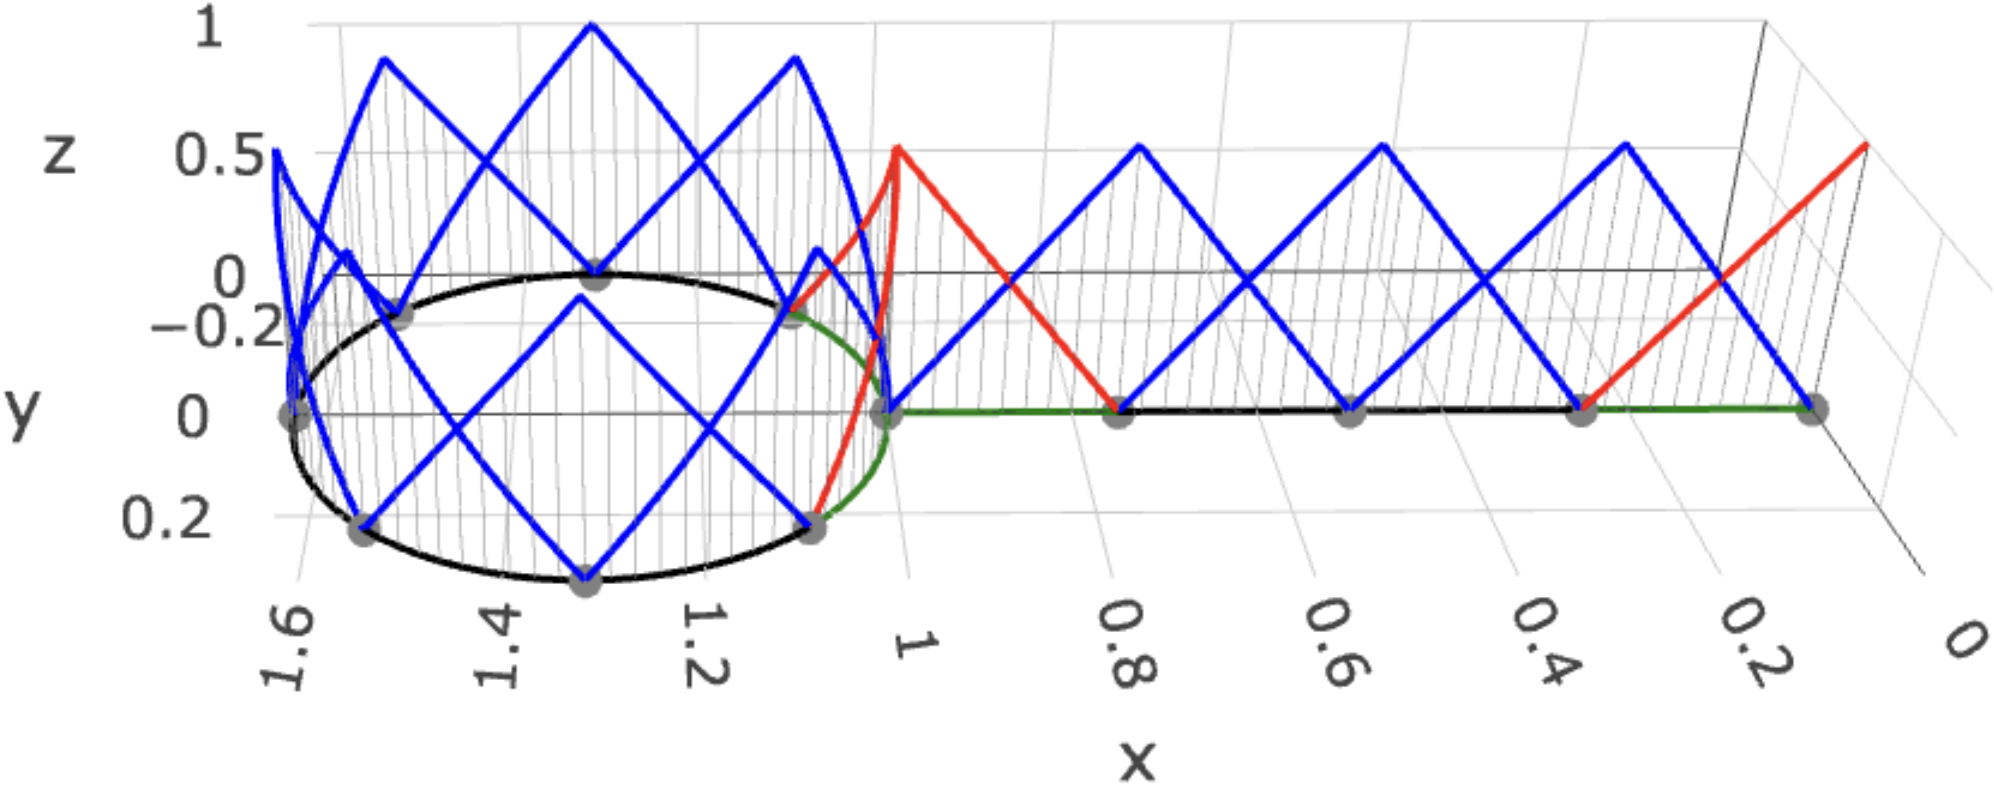
\includegraphics[width=0.4\textwidth]{Fig/basis2.png}
\caption{Illustration of the basis function system $\{\psi^i_h\}_{i=1}^{N_h}$ on the tadpole graph (in black). Standard hat functions associated with internal edge nodes are shown in blue, while vertex-centered functions are highlighted in red. The star-shaped structures around the vertices are shown in green.}
\label{basis}
\end{figure}


To approximate the fractional operator, we introduce the discrete operator on $V_h$.
\begin{definition}
   We define the discrete version of $L$ as $L_h:V_h\to V_h$ via $(L_h\phi,\psi)_{L_2(\Gamma)} = a(\phi, \psi)$ for all $\phi,\psi\in V_h$, where $a:H^1(\Gamma)\times H^1(\Gamma)\to\mathbb{R}$ given by $a(u,v)= \kappa^2(u,v)_{L_2(\Gamma)} + (u',v')_{L_2(\Gamma)}$ is the bilinear form associated with $L$.
\end{definition}
Since $L_h$ is symmetric positive definite on $V_h$, it admits a spectral decomposition with eigenpairs $\{(\lambda_{j,h},e_{j,h})\}_{j=1}^{N_h}$. The eigenfunctions $\{e_{j,h}\}_{j=1}^{N_h}$ are orthonormal in $L_2(\Gamma)$, while the eigenvalues satisfy $0<\kappa^2=\lambda_{1,h}\leq\cdots\leq\lambda_{N_h,h}$ and $\lambda_j\leq\lambda_{j,h}$ for $j=1,\dots,N_h$ \cite[Section~6.3]{bolin2023regularity}. For $\alpha\in[0,2]$, we define the fractional power of $L_h$ by $L_h^{\sfrac{\alpha}{2}}\phi=\sum_{j=1}^{N_h}\lambda_{j,h}^{\sfrac{\alpha}{2}}(\phi,e_{j,h})_{L_2(\Gamma)}e_{j,h}$ for $\phi\in V_h$. This induces the discrete bilinear form $\mathfrak{a}_{h,\alpha}:V_h\times V_h\to\mathbb{R}$, given by $\mathfrak{a}_{h,\alpha}(\phi,\psi)=(L_h^{\sfrac{\alpha}{4}}\phi,L_h^{\sfrac{\alpha}{4}}\psi)_{L_2(\Gamma)}$ for $\phi,\psi\in V_h$.
\subsection{Elliptic projection}
In this subsection, we introduce the $L_2(\Gamma)$-orthogonal projector $P_h$ and the elliptic projector $G_{h,\alpha}$. While $P_h$ provides optimal approximation properties in $L_2(\Gamma)$, the operator $G_{h,\alpha}$ is defined via the bilinear form $\mathfrak{a}_{\alpha}(\cdot,\cdot)$ and plays a central role in the error analysis of the discrete fractional operator.

\begin{definition}
Let $P_h:L_2(\Gamma)\to V_h$ denote the $L_2(\Gamma)$-orthogonal projection onto $V_h$, i.e., for $\phi\in L_2(\Gamma)$, the projection $P_h\phi$ is the unique function in $V_h$ satisfying $(P_h\phi,v_h)_{L_2(\Gamma)} = (\phi,v_h)_{L_2(\Gamma)}$ for all $v_h\in V_h$.
\end{definition}
\begin{definition}
Let $\alpha\in[0,2]$. For $\alpha=0$, we define $G_{h,0}:=P_h$. For $\alpha\in(0,2]$ and $\phi\in\dot{H}^{\sfrac{\alpha}{2}}(\Gamma)$, the elliptic projector $G_{h,\alpha}:\dot{H}^{\sfrac{\alpha}{2}}(\Gamma)\to V_h$ is such that $G_{h,\alpha}\phi\in V_h$ is unique and
\begin{align}
\label{eq:elliptic_projector}
        \mathfrak{a}_{\alpha}(G_{h,\alpha}\phi,v_h) = \mathfrak{a}_{\alpha}(\phi,v_h),\quad\forall v_h\in V_h.
\end{align}

\end{definition}
\begin{proposition}
\label{proposition:with_projection}
    Let $\alpha\in[0,2]$. If $\phi\in\dot{H}^{\alpha}(\Gamma)$, then $\|\phi-P_h \phi\|_{L_2(\Gamma)}\lesssim h^{\alpha}\|\phi\|_{\dot{H}^{\alpha}(\Gamma)}$.
\end{proposition}
\begin{proof}
    Since $P_h$ is the $L_2(\Gamma)$-orthogonal projection, we have $\|(I-P_h)\phi\|_{L_2(\Gamma)}\leq\|\phi\|_{L_2(\Gamma)}$. This corresponds to the estimate with $\alpha = 0$. By definition of $P_h$ and \cite[Proposition~6.2]{bolin2023regularity}, we obtain $\|(I-P_h)\phi\|_{L_2(\Gamma)}\leq\|(I-G_{h,2})\phi\|_{L_2(\Gamma)}\leq h^2\|\phi\|_{\dot{H}^2(\Gamma)}$, which yields the estimate with $\alpha = 2$. Having obtained the estimate for $\alpha = 0$ and $\alpha=2$, we can apply the interpolation theory from \cite[Section~3.2]{ChandlerWilde2015interpolation} (specifically,  Theorem 3.5 and (ii) on page 428 with $T=I-P_h$) to obtain estimate for $\alpha\in[0,2]$ as well. %This concludes the proof.
    \hfill
\end{proof}
\begin{lemma}
\label{lem:graph-fractional-fe-approx}
    If $\mathcal{T}_h$ is quasi-uniform, then for every $0\leq t\leq1$ and $t\leq s\leq2$, we have $\inf_{v_h\in V_h}\|u-v_h\|_{\dot H^t(\Gamma)}\lesssim h^{s-t}\|u\|_{\dot H^s(\Gamma)}$ for all $u\in \dot H^s(\Gamma)$. In particular, for every $\alpha\in(0,2]$, we have $\inf_{v_h\in V_h}\|u-v_h\|_{\dot H^{\sfrac{\alpha}{2}}(\Gamma)}\lesssim h^{\sfrac{\alpha}{2}}\|u\|_{\dot H^\alpha(\Gamma)}$ for all $u\in \dot H^\alpha(\Gamma)$.
\end{lemma}
\begin{proof}
    We first prove the estimate for $0\leq t\leq s\leq1$. Since $\dot H^1(\Gamma)=H^1(\Gamma)$ with equivalent norms, the spectral characterization of $L$ implies that it suffices to prove the result for the interpolation scale $H^r(\Gamma)=[L_2(\Gamma),H^1(\Gamma)]_r$, $0\le r\le1$. For each node $a\in\mathcal N_h$, fix once and for all a mesh interval $K_a\in\mathcal T_h$ having $a$ as an endpoint. If several such intervals exist, choose one arbitrarily. For each node $a\in\mathcal N_h$, let $\psi_a\in V_h$ be the associated global hat function, let $\ell_a = \psi_a|_{K_a}$ denote the local affine nodal basis function on $K_a$ corresponding to $a$, and let $\eta_a\in\mathbb P_1(K_a)$ be the local dual basis function satisfying $\int_{K_a}\eta_a\ell_b\dd x=\delta_{ab}$ for each endpoint $b$ of $K_a$. Define the linear functional $\lambda_a(u)=\int_{K_a}u\,\eta_a\dd x$ for $u\in L_2(\Gamma)$ and define the quasi-interpolant $\Pi_hu=\sum_{a\in\mathcal N_h}\lambda_a(u)\psi_a$. Then $\Pi_h:L_2(\Gamma)\to V_h$ is well-defined. Moreover, $\Pi_h$ reproduces $V_h$. Indeed, if $v_h\in V_h$, then $v_h|_{K_a}$ is affine and therefore $\lambda_a(v_h)=v_h(a)$. Since $v_h$ is continuous at graph vertices, this value is independent of the edge by which the vertex is approached. Hence $\Pi_hv_h=\sum_{a\in\mathcal N_h}v_h(a)\psi_a=v_h$. For each interval $K\in\mathcal T_h$, denote its endpoints by $a_K$ and $b_K$ and define $\omega_K=K\cup K_{a_K}\cup K_{b_K}$. This is a connected subgraph of $\Gamma$. It consists of at most three mesh intervals and satisfies $|\omega_K|\leq (1+2\rho)h_K$. Let $D_\Gamma:=\max\{2,\max_{v\in\mathcal V}\deg(v)\}$. Thus, every mesh node is contained in at most $D_\Gamma$ mesh intervals. Furthermore, each fixed mesh interval $J\in\mathcal T_h$ is contained in at most $N_{\mathrm{ov}}:=1+2D_\Gamma$ of the patches $\omega_K$.

    Next we prove $L_2$ stability. On the reference interval $(0,1)$, the two dual functions to the affine nodal basis have finite $L_2$ norms. By scaling, $\|\eta_a\|_{L_2(K_a)}\lesssim h_{K_a}^{-\sfrac{1}{2}}$ and consequently, $|\lambda_a(u)|\lesssim h_{K_a}^{-\sfrac{1}{2}}\|u\|_{L_2(K_a)}$. On any interval $K$ with endpoint $a$, the restriction of $\psi_a$ is affine and satisfies $\|\psi_a\|_{L_2(K)}\leq h_K^{\sfrac{1}{2}}$ and $\|\psi_a'\|_{L_2(K)}\leq h_K^{-\sfrac{1}{2}}$. By quasi-uniformity, $h_K/h_{K_a}\leq\rho$, whenever $a$ is an endpoint of $K$. Therefore, $\|\Pi_hu\|_{L_2(K)} \leq |\lambda_{a_K}(u)|\|\psi_{a_K}\|_{L_2(K)} + |\lambda_{b_K}(u)|\|\psi_{b_K}\|_{L_2(K)} \lesssim \rho^{\sfrac{1}{2}}\|u\|_{L_2(\omega_K)}$. After squaring and summing over $K$, and using the overlap bound
    $N_{\mathrm{ov}}$, we obtain $\|\Pi_hu\|_{L_2(\Gamma)}\lesssim\|u\|_{L_2(\Gamma)}$.

    Next we prove $H^1$ stability. Since $\Pi_h$ reproduces constants, for any constant $c$, we have $(\Pi_hu)'=(\Pi_h(u-c))'$. Using the derivative estimate above gives $\|(\Pi_hu)'\|_{L_2(K)}\lesssim h_K^{-1}\|u-c\|_{L_2(\omega_K)}$. Let $c_{\mathrm{av}}$ denote the average of $u$ over $\omega_K$. Since $\omega_K$ is connected, the Poincare inequality on a connected one-dimensional metric graph gives $ \|u-c_{\mathrm{av}}\|_{L_2(\omega_K)} \leq|\omega_K|\,\|u'\|_{L_2(\omega_K)}$. Indeed, for almost every $x,y\in\omega_K$, continuity on the connected patch and integration along a path in $\omega_K$ joining $x$ and $y$ imply $|u(x)-u(y)|\leq|\omega_K|^{\sfrac{1}{2}}\|u'\|_{L_2(\omega_K)}$, and the above Poincare inequality follows by averaging in $y$ and then integrating in $x$. Therefore, $\|(\Pi_hu)'\|_{L_2(K)}\lesssim h_K^{-1}|\omega_K|\|u'\|_{L_2(\omega_K)}\lesssim(1+2\rho)\|u'\|_{L_2(\omega_K)}$. Squaring and summing over $K$, again using the overlap bound $N_{\mathrm{ov}}$, yields $\|(\Pi_hu)'\|_{L_2(\Gamma)}\lesssim\|u'\|_{L_2(\Gamma)}$. Together with the $L_2$ stability, this gives $\|\Pi_hu\|_{H^1(\Gamma)}\lesssim\|u\|_{H^1(\Gamma)}$.

    Let $E_h=I-\Pi_h$. Since $\Pi_h$ reproduces constants, $E_hu=(u-c_{\mathrm{av}})-\Pi_h(u-c_{\mathrm{av}})$. Hence, by the local $L_2$ stability of $\Pi_h$ and the Poincare inequality on $\omega_K$, we have $\|E_hu\|_{L_2(K)}\lesssim \|u-c_{\mathrm{av}}\|_{L_2(\omega_K)}\lesssim h_K\|u'\|_{L_2(\omega_K)}$.  Squaring, summing over $K$, and using the overlap bound gives $\|E_hu\|_{L_2(\Gamma)}\lesssim h\|u\|_{H^1(\Gamma)}$. By the $L_2$- and $H^1$-stability of $\Pi_h$, we also have that $E_h:L_2(\Gamma)\to L_2(\Gamma)$ and $E_h: H^1(\Gamma)\to H^1(\Gamma)$ are bounded. By interpolation in the target space, for every $0\leq t\leq1$, we have $\|E_hu\|_{H^t(\Gamma)}\lesssim h^{1-t}\|u\|_{H^1(\Gamma)}$. Also, interpolation of the $L_2$ and $H^1$ stability estimates gives $\|E_hu\|_{H^t(\Gamma)}\lesssim\|u\|_{H^t(\Gamma)}$. Fix $0\leq t\leq s\leq1$. If $s=t$, the desired bound follows from the last estimate. If $t<s\leq1$, interpolate the two mappings $E_h:H^t(\Gamma)\to H^t(\Gamma)$ and $E_h:H^1(\Gamma)\to H^t(\Gamma)$. Since $H^s(\Gamma)=[H^t(\Gamma),H^1(\Gamma)]_\theta$ for $\theta=(s-t)/(1-t)$, we obtain $\|E_hu\|_{H^t(\Gamma)}\lesssim h^{\theta(1-t)}\|u\|_{H^s(\Gamma)}= h^{s-t}\|u\|_{H^s(\Gamma)}$. Returning to the equivalent spectral norms gives $\|u-\Pi_hu\|_{\dot H^t(\Gamma)}\lesssim h^{s-t}\|u\|_{\dot H^s(\Gamma)}$ for $0\leq t\leq s\leq1$.

    It remains to treat the case $1\leq s\leq2$ and $0\leq t\leq1$. In this range we use the nodal interpolant $I_hu\in V_h$. This is well-defined because $\dot H^s(\Gamma)\subset H^1(\Gamma)$ for $s\geq1$, and functions in $H^1(\Gamma)$ are continuous on the metric graph. Let $F_h = I-I_h$. On each mesh interval $K=[x_0,x_1]$, the restriction of $I_hu$ is the affine interpolant of $u|_K$ at the endpoints. For $u\in H^1(\Gamma)$, we have $(I_hu)'|_K = (u(x_1)-u(x_0))/h_K= h_K^{-1}\int_K u'(x)\dd x$. Hence, $\|(I_hu)'\|_{L_2(K)}\leq\|u'\|_{L_2(K)}$ and $ \|(F_hu)'\|_{L_2(K)}\lesssim\|u'\|_{L_2(K)}$. Moreover, since $F_hu$ vanishes at the endpoints of $K$, we have $\|F_hu\|_{L_2(K)}\leq h_K\|(F_hu)'\|_{L_2(K)}\lesssim h_K\|u'\|_{L_2(K)}$. After summing over $K$, we obtain $\|F_hu\|_{L_2(\Gamma)}\lesssim h\|u\|_{\dot H^1(\Gamma)}$ and  $\|F_hu\|_{\dot H^1(\Gamma)}\lesssim\|u\|_{\dot H^1(\Gamma)}$. For $u\in\dot H^2(\Gamma)=D(L)$, we have $u|_e\in H^2(e)$ on each edge $e$ and $        \sum_{e}\|u_e''\|_{L_2(e)}^2\lesssim\|u\|_{\dot H^2(\Gamma)}^2$. Indeed, edgewise, $Lu=\kappa^2u-u''$, and hence $\|u''\|_{L_2(\Gamma)}\leq\|Lu\|_{L_2(\Gamma)}+\kappa^2\|u\|_{L_2(\Gamma)}\lesssim\|u\|_{\dot H^2(\Gamma)}$. The standard one-dimensional interpolation estimates on each mesh interval give $\|F_hu\|_{L_2(K)}\lesssim h_K^2\|u''\|_{L_2(K)}$ and $\|(F_hu)'\|_{L_2(K)}\lesssim h_K\|u''\|_{L_2(K)}$. Summing over $K$ yields $\|F_hu\|_{L_2(\Gamma)}\lesssim h^2\|u\|_{\dot H^2(\Gamma)}$ and $\|F_hu\|_{\dot H^1(\Gamma)}\lesssim h\|u\|_{\dot H^2(\Gamma)}$. Interpolating between the endpoint estimates $I-I_h:\dot H^1(\Gamma)\to L_2(\Gamma)$ and $I-I_h:\dot H^2(\Gamma)\to L_2(\Gamma)$ gives $\|F_hu\|_{L_2(\Gamma)}\lesssim h^s\|u\|_{\dot H^s(\Gamma)} $ for $1\leq s\leq2$. Similarly, interpolating $I-I_h:\dot H^1(\Gamma)\to \dot H^1(\Gamma)$ and $I-I_h:\dot H^2(\Gamma)\to \dot H^1(\Gamma)$ gives $\|F_hu\|_{\dot H^1(\Gamma)}\lesssim h^{s-1}\|u\|_{\dot H^s(\Gamma)}$ for $1\leq s\leq2$. Finally, for $0\leq t\leq1$, the interpolation inequality in the Hilbert scale generated by $L$ gives 
    \begin{align*}
        \|F_hu\|_{\dot H^t(\Gamma)}
        \lesssim
        \|F_hu\|_{L_2(\Gamma)}^{1-t}
        \|F_hu\|_{\dot H^1(\Gamma)}^t  \lesssim h^{s-t}\|u\|_{\dot H^s(\Gamma)} .
    \end{align*}
    Since $I_hu\in V_h$, this also proves the desired best-approximation estimate for $1\leq s\leq2$.
    \hfill
\end{proof}
\begin{proposition}
\label{proposition:with_elliptic_projection}
Let $\alpha\in[0,2]$. If $\phi\in\dot{H}^{\alpha}(\Gamma)$, then $\|\phi - G_{h,\alpha}\phi\|_{L_2(\Gamma)} \lesssim h^\alpha\|\phi\|_{\dot{H}^{\alpha}(\Gamma)}$.
\end{proposition}
\begin{proof}
    Let $\alpha\in(0,2]$ and $e_h=\phi-G_{h,\alpha}\phi$. By using \eqref{eq:elliptic_projector}, the Galerkin orthogonality relation $\mathfrak{a}_{\alpha}(e_h,v_h)=0$ holds for every $v_h\in V_h$. Since $\mathfrak{a}_{\alpha}$ is the inner product on $\dot H^{\sfrac{\alpha}{2}}(\Gamma)$, $G_{h,\alpha}$ is the $\mathfrak{a}_{\alpha}$-orthogonal projection onto $V_h$. Therefore, for any $v_h\in V_h$, writing $e_h=(\phi-v_h)+(v_h-G_{h,\alpha}\phi)$ and observing that $v_h-G_{h,\alpha}\phi\in V_h$, we have $\|e_h\|_{\dot H^{\sfrac{\alpha}{2}}(\Gamma)}^2 =\mathfrak{a}_{\alpha}(e_h,e_h) =\mathfrak{a}_{\alpha}(e_h,\phi-v_h) \leq \|e_h\|_{\dot H^{\sfrac{\alpha}{2}}(\Gamma)} \|\phi-v_h\|_{\dot H^{\sfrac{\alpha}{2}}(\Gamma)}$. This and Lemma~\ref{lem:graph-fractional-fe-approx} imply
    \begin{align}
    \label{ineq:energy_estimate}
    \textstyle
        \|e_h\|_{\dot H^{\sfrac{\alpha}{2}}(\Gamma)}\leq\inf_{v_h\in V_h}\|\phi-v_h\|_{\dot H^{\sfrac{\alpha}{2}}(\Gamma)}\lesssim h^{\sfrac{\alpha}{2}}\|\phi\|_{\dot H^\alpha(\Gamma)}.
    \end{align}
    We now use a duality argument. Let $z\in\dot H^\alpha(\Gamma)$ solve $\mathfrak{a}_{\alpha}(z,v)=(e_h,v)_{L_2(\Gamma)}$ for all $v\in \dot H^{\sfrac{\alpha}{2}}(\Gamma)$. By elliptic regularity (Proposition \ref{proposition:elliptic_regularity} with $r=0$, $u = z$, and $f=e_h$), we have $\|z\|_{\dot H^\alpha(\Gamma)} = \|e_h\|_{L_2(\Gamma)}$. Taking $v=e_h$ and letting $z_h\in V_h$ be arbitrary, the symmetry of $\mathfrak{a}_{\alpha}$ and Galerkin orthogonality yield $\|e_h\|_{L_2(\Gamma)}^2 = \mathfrak{a}_{\alpha}(e_h,z-z_h)\leq\|e_h\|_{\dot H^{\sfrac{\alpha}{2}}(\Gamma)}\|z-z_h\|_{\dot H^{\sfrac{\alpha}{2}}(\Gamma)}$. This and Lemma~\ref{lem:graph-fractional-fe-approx} imply
    \begin{align*}
    \textstyle
        \|e_h\|_{L_2(\Gamma)}^2 \leq \|e_h\|_{\dot H^{\sfrac{\alpha}{2}}(\Gamma)} \inf_{z_h\in V_h}\|z-z_h\|_{\dot H^{\sfrac{\alpha}{2}}(\Gamma)} \lesssim h^{\sfrac{\alpha}{2}} \|e_h\|_{\dot H^{\sfrac{\alpha}{2}}(\Gamma)} \|z\|_{\dot H^\alpha(\Gamma)} 
    \end{align*}
    By \eqref{ineq:energy_estimate} and the identity $\|z\|_{\dot H^\alpha(\Gamma)} = \|e_h\|_{L_2(\Gamma)}$, we get $\|e_h\|_{L_2(\Gamma)}^2\lesssim h^\alpha \|\phi\|_{\dot H^\alpha(\Gamma)}\|e_h\|_{L_2(\Gamma)}$. If $e_h\neq0$, division by $\|e_h\|_{L_2(\Gamma)}$ yields the estimate. If $e_h=0$, the estimate is immediate. Finally, since $G_{h,0}=P_h$ by convention, then for $\alpha=0$ the
estimate becomes $\|\phi-P_h\phi\|_{L_2(\Gamma)}\leq\|\phi\|_{L_2(\Gamma)}$, which is the stability of the $L_2(\Gamma)$-orthogonal projection.
\hfill
\end{proof}
\begin{lemma}
    \label{lemma:boundwithhminus2}
    If $\mathcal{T}_h$ is quasi-uniform, then $\|L_h\phi\|_{L_2(\Gamma)}\lesssim h^{-2}\|\phi\|_{L_2(\Gamma)}$ for $\phi\in V_h$.
\end{lemma}
\begin{proof}
    Since $L_h \phi \in V_h$, it follows that  $\left\|L_h \phi\right\|_{L_2(\Gamma)}=\sup _{\substack{\psi \in V_h :\|\psi\|_{L_2(\Gamma)}=1}} a(\phi, \psi)$. Under quasi-uniformity, the inverse inequality yields
        \begin{align*}
            a(\phi, \psi) \leq\|\phi\|_{\dot{H}^1(\Gamma)}\|\psi\|_{\dot{H}^1(\Gamma)} \lesssim(h^{-1}\|\phi\|_{L_2(\Gamma)})(h^{-1}\|\psi\|_{L_2(\Gamma)})=h^{-2}\|\phi\|_{L_2(\Gamma)}.
        \end{align*}
        Taking the supremum gives the result.
        \hfill
\end{proof}
\begin{proposition}
\label{prop:controlofLhbyL}
        Let $\alpha\in[0,2]$. If $\phi\in\dot{H}^{\alpha}(\Gamma)$, then $\|L_h^{\sfrac{\alpha}{2}}P_h\phi\|_{L_2(\Gamma)} \lesssim \|L^{\sfrac{\alpha}{2}}\phi\|_{L_2(\Gamma)}$.
\end{proposition}
\begin{proof}
     For $\alpha = 0$, the result is immediate. For $\alpha = 2$, let $\phi\in D(L) = \dot{H}^2(\Gamma)$ and $v_h\in V_h$. It follows that $(L_hG_{h,2}\phi,v_h)_{L_2(\Gamma)} = \mathfrak{a}_{2}(G_{h,2}\phi,v_h)  = \mathfrak{a}_{2}(\phi,v_h)  = (L\phi,v_h)_{L_2(\Gamma)} = (P_hL\phi,v_h)_{L_2(\Gamma)}$. Since this holds for all $v_h\in V_h$, we have that $L_hG_{h,2}\phi = P_hL\phi$ for all $\phi\in \dot{H}^2(\Gamma)$. This and the contraction property of $P_h$ yields $\|L_hP_h\phi\|_{L_2(\Gamma)} \leq \|L\phi\|_{L_2(\Gamma)}  +  \|L_h(P_h\phi - G_{h,2}\phi)\|_{L_2(\Gamma)}$. Since $P_h\phi - G_{h,2}\phi\in V_h$, Lemma \ref{lemma:boundwithhminus2} implies that $\|L_h(P_h\phi - G_{h,2}\phi)\|_{L_2(\Gamma)}  \lesssim h^{-2}\|P_h\phi - G_{h,2}\phi\|_{L_2(\Gamma)}$. By Propositions \ref{proposition:with_projection} and \ref{proposition:with_elliptic_projection}, we have that $\|P_h\phi - G_{h,2}\phi\|_{L_2(\Gamma)}  \lesssim h^2\|L\phi\|_{L_2(\Gamma)} + h^2\|L\phi\|_{L_2(\Gamma)}$. By combining the previous three inequalities, we obtain the estimate with $\alpha=2$. It remains to consider $0<\alpha<2$. Let $\beta=\sfrac{\alpha}{2}$. We use interpolation between the cases $\alpha=0$ and $\alpha=2$. The two endpoint estimates show that $P_h:(L_2(\Gamma),\|\cdot\|_{L_2(\Gamma)})\to (V_h,\|\cdot\|_{L_2(\Gamma)})$ and $P_h:(D(L),\|L\cdot\|_{L_2(\Gamma)})\to (V_h,\|L_h\cdot\|_{L_2(\Gamma)})$ are bounded uniformly in $h$. Therefore, $P_h$ is a bounded couple map (see \cite{ChandlerWilde2015interpolation}), and for every $0<\beta<1$, $P_h:[L_2(\Gamma),D(L)]_\beta\to[V_h,V_h]_\beta$ is bounded uniformly in $h$. Since $L$ and $L_h$ are positive self-adjoint operators, \cite[Theorem~4.36]{Lunardi2018Interpolation} yields $[L_2(\Gamma),D(L)]_\beta=D(L^\beta)$ and $[V_h,V_h]_\beta=D(L_h^\beta)=V_h$, where the interpolation norms are equivalent to the corresponding graph norms. Moreover, since the spectra of $L$ and $L_h$ are bounded below by $\kappa^2>0$, these graph norms are equivalent to $\|L^\beta\cdot\|_{L_2(\Gamma)}$ and $\|L_h^\beta\cdot\|_{L_2(\Gamma)}$, respectively. Consequently, for every $\phi\in D(L^\beta)$, we have $\|L_h^\beta P_h\phi\|_{L_2(\Gamma)}\lesssim\|L^\beta\phi\|_{L_2(\Gamma)}$. %This finishes the proof.
     \hfill
    \end{proof}

        
            
We now introduce both semidiscrete and fully discrete schemes for approximating the solution to problem~\eqref{weakformofentireequation}.
%
Let $\alpha>0$ and $U^\tau$ denote the sequence of time-discrete approximations of the solution to problem \eqref{weakformofentireequation}. The scheme~\eqref{system:semidiscrete_scheme}, referred to as the \emph{semidiscrete scheme}, determines the sequence $U^\tau$ of elements of $\dot{H}^{\sfrac{\alpha}{2}}(\Gamma)$ by requiring that the iterate $U^{k+1}$ satisfies
\begin{equation}
\label{system:semidiscrete_scheme}
    \left\{
\begin{aligned}
    \langle\delta U^{k+1},\phi\rangle + \mathfrak{a}_{\alpha}(U^{k+1},\phi)  &= \langle f^{k+1},\phi\rangle , \quad\forall\phi\in \dot{H}^{\sfrac{\alpha}{2}}(\Gamma),\quad k=0,\dots, N-1, \\
    U^0 &= u_0.
\end{aligned}
\right.
\end{equation}

We now extend the construction to include spatial discretization. Let $\alpha\in(0,2]$ and $U_h^\tau$ denote the sequence of approximations of the solution to problem \eqref{weakformofentireequation} at each time step on a mesh indexed by $h$. The scheme~\eqref{system:fully_discrete_scheme}, referred to as the \emph{fully discrete scheme}, determines $U_h^{\tau}\subset V_h$ by requiring that the iterate $U^{k+1}_h$ satisfies
\begin{equation}
\label{system:fully_discrete_scheme}
    \left\{
\begin{aligned}
    \langle\delta U_h^{k+1},\phi\rangle + \mathfrak{a}_{h,\alpha}(
        U_h^{k+1},\phi) &= \langle f^{k+1},\phi\rangle, \quad\forall\phi\in V_h,\quad k=0,\dots, N-1, \\
    U^0_h &= P_hu_0.
\end{aligned}
\right.
\end{equation}
\section{Time and space error analysis}
\label{timeandspaceerroranalysis}
In this section, we derive rigorous error estimates that quantify the accuracy of the numerical scheme with respect to both temporal and spatial discretizations.
\begin{theorem}
\label{theorem:first_part_of_main}
    Let $\alpha>0$ and $u$ be the solution to \eqref{weakformofentireequation}. Let $\tilde{U}^\tau$ be the piecewise constant function (defined via \eqref{def:piecewise_constant}) constructed from the solution to \eqref{system:semidiscrete_scheme}. If $u_0\in\dot{H}^{\sfrac{\alpha}{2}}(\Gamma)$ and $f\in L_2(0,T;L_2(\Gamma))$, then $\|u-\tilde{U}^\tau\|_{L_2(0,T;L_2(\Gamma))}\lesssim \tau$.
\end{theorem}
\begin{proof}
The proof follows the same arguments as in \cite[Theorem~5.6]{Glusa2021errorestimates}, with the obvious adaptations to the metric graph setting and the corresponding variational framework on $\Gamma$. We therefore omit the details.
\hfill
\end{proof}
\begin{theorem}
\label{theorem:theorem_second_part_of_main}
Let $\alpha\in(0,2]$ and $U^\tau$ and $U_h^\tau$ be the solutions to \eqref{system:semidiscrete_scheme} and \eqref{system:fully_discrete_scheme}, respectively. If $u_0\in\dot{H}^{\sfrac{\alpha}{2}}(\Gamma)$ and $f\in L_2(0,T;L_2(\Gamma))$, then, for sufficiently small $\epsilon>0$, we have $\|U^\tau-U_h^\tau\|_{\ell^2(L_2(\Gamma))}\lesssim h^{\alpha-\epsilon}$. For $\alpha=2$, the estimate holds with $\epsilon=0$.
\end{theorem}

\begin{proof}  
    For convenience, write $H=L_2(\Gamma)$ and $\beta=\sfrac{\alpha}{2}$. The semidiscrete scheme \eqref{system:semidiscrete_scheme} implies $L^\beta U^{k+1}=f^{k+1}- \delta U^{k+1}$ in $\dot H^{-\beta}(\Gamma)$. Since $f^{k+1}- \delta U^{k+1}\in H$, Proposition~\ref{proposition:elliptic_regularity} with $r=0$ yields $U^{k+1}\in\dot H^{2\beta}(\Gamma)$ for $k = 0,\dots,N-1$, and the equation holds in $H$. Likewise, the fully discrete scheme \eqref{system:fully_discrete_scheme} holds in $V_h$. Thus both schemes admit strong forms, given by
    \begin{align}
    \label{eq:alternative_strong_schemes}
    \delta U^{k+1}+L^\beta U^{k+1}=f^{k+1}\quad\text{ and }\quad
    \delta U_h^{k+1}+L_h^\beta U_h^{k+1}=P_hf^{k+1},
    \end{align}
    with $U^0=u_0$ and $U_h^0=P_hu_0$. To compare the inverse operators, set
    \begin{align*}
        A=L^{-\beta}:H\to H, \qquad B_h=L_h^\beta:V_h\to V_h, \qquad D_h=A-B_h^{-1}P_h:H\to H.
    \end{align*}
    By \cite[Lemma~6.4(a)]{bolin2023regularity}, taking $s=0$ in their notation, we obtain
    \begin{align}
    \label{eq:alternative_inverse_bound}
    \|D_h\|_{\mathcal L(H)}
    =\|L^{-\beta}-L_h^{-\beta}P_h\|_{\mathcal L(H)}
    \lesssim h^{2\beta-\epsilon}.
    \end{align}
    for $0<\beta<1$ and sufficiently small $\epsilon>0$. For $\beta=1$, the same bound with $\epsilon=0$ follows from the ordinary elliptic projection estimate.
    
    We now estimate the discrete time derivative. Taking the $H$-inner product of the second equation in~\eqref{eq:alternative_strong_schemes} with $\delta U_h^{k+1}$ yields
    \begin{align*}
    \|\delta U_h^{k+1}\|_H^2
    +(B_hU_h^{k+1},\delta U_h^{k+1})_H
    =(f^{k+1},\delta U_h^{k+1})_H.
    \end{align*}
    By self-adjointness of $B_h$, and the identity $2(a,a-b)=\|a\|^2-\|b\|^2+\|a-b\|^2$ applied to $a=B_h^{\sfrac12}U_h^{k+1}$ and $b=B_h^{\sfrac12}U_h^k$, we obtain, after dropping terms
    \begin{align*}
    (B_hU_h^{k+1},\delta U_h^{k+1})_H
    \geq(2\tau)^{-1}\|B_h^{\sfrac12}U_h^{k+1}\|_H^2-(2\tau)^{-1}\|B_h^{\sfrac12}U_h^k\|_H^2.
    \end{align*}
    Cauchy--Schwarz and the inequality $ab\leq(a^2+b^2)/2$ yield
    \begin{align*}
    (f^{k+1},\delta U_h^{k+1})_H
    \leq2^{-1}\|f^{k+1}\|_H^2+2^{-1}\|\delta U_h^{k+1}\|_H^2.
    \end{align*}
    We combine the previous three expressions to arrive at
    \begin{align*}
    2^{-1}\|\delta U_h^{k+1}\|_H^2
    +(2\tau)^{-1}\|B_h^{\sfrac12}U_h^{k+1}\|_H^2-(2\tau)^{-1}\|B_h^{\sfrac12}U_h^k\|_H^2
    \leq2^{-1}\|f^{k+1}\|_H^2.
    \end{align*}
    Multiplying by $2\tau$ and summing over $k=0,\ldots,N-1$, we obtain, by telescoping,
    \begin{align*}
    \textstyle
    \tau\sum_{k=0}^{N-1}\|\delta U_h^{k+1}\|_H^2
    +\|B_h^{\sfrac12}U_h^N\|_H^2
    \leq\tau\sum_{k=0}^{N-1}\|f^{k+1}\|_H^2
    +\|B_h^{\sfrac12}P_hu_0\|_H^2.
    \end{align*}
    Dropping terms and applying Jensen's inequality and Proposition~\ref{prop:controlofLhbyL} yields
    \begin{align}
    \label{eq:alternative_time_derivative}
    \textstyle
    \tau\sum_{k=0}^{N-1}\|\delta U_h^{k+1}\|_H^2
    \lesssim\|f\|_{L_2(0,T;H)}^2+\|u_0\|_{\dot H^\beta(\Gamma)}^2.
    \end{align}

    We now derive the error equation. Let $e^k = U^{k}-U_h^{k}$. Multiplying the first equation in~\eqref{eq:alternative_strong_schemes} by $A=L^{-\beta}$ and the second by $B_h^{-1}$ and then subtracting yields
    \begin{align*}
    A\delta U^{k+1}-B_h^{-1}\delta U_h^{k+1}+e^{k+1}
    =D_hf^{k+1}.
    \end{align*}
    Let $g^{k+1}=D_h(f^{k+1}-\delta U_h^{k+1})$ for $k=0,\ldots,N-1$. By linearity of the difference quotient, and since $P_h\delta U_h^{k+1}=\delta U_h^{k+1}$, we have $A\delta U^{k+1}-B_h^{-1}\delta U_h^{k+1}
    =A\delta e^{k+1}+D_h\delta U_h^{k+1}$. By replacing this in the previous expression, we obtain the error equation
    \begin{align}
    \label{eq:alternative_error_equation}
    A\delta e^{k+1}+e^{k+1}=g^{k+1},\quad e^0=(I-P_h)u_0.
    \end{align}
    To derive an energy estimate for the error, we take the $H$-inner product of~\eqref{eq:alternative_error_equation} with $e^{k+1}$ and repeat the energy argument above, now with $A^{\sfrac12}e^{k+1}$ and $A^{\sfrac12}e^k$. Using positivity and self-adjointness of $A$, summing in time, and dropping terms, we obtain 
    \begin{align} 
    \label{eq:alternative_error_energy}
    \textstyle
    \tau\sum_{k=0}^{N-1}\|e^{k+1}\|_H^2
    \leq\tau\sum_{k=0}^{N-1}\|g^{k+1}\|_H^2+\|A^{\sfrac12}(I-P_h)u_0\|_H^2.
    \end{align}
    
    We now estimate the first term on the right-hand side of~\eqref{eq:alternative_error_energy}. By the definition of $g^{k+1}$ and~\eqref{eq:alternative_inverse_bound}, we have $\|g^{k+1}\|_H \lesssim h^{2\beta-\epsilon} \left(\|f^{k+1}\|_H+\|\delta U_h^{k+1}\|_H\right)$. Squaring, using $(a+b)^2\leq2a^2+2b^2$, multiplying by $\tau$, and summing yields
    \begin{align*}
    \textstyle
    \tau\sum_{k=0}^{N-1}\|g^{k+1}\|_H^2
    \lesssim h^{2(2\beta-\epsilon)}
    \big(\tau\sum_{k=0}^{N-1}\|f^{k+1}\|_H^2
    +\tau\sum_{k=0}^{N-1}\|\delta U_h^{k+1}\|_H^2\big).
    \end{align*}
    The first sum is bounded by Jensen's inequality, and the second by~\eqref{eq:alternative_time_derivative}. Therefore,
    \begin{align}
    \label{eq:alternative_forcing_bound}
    \textstyle
    \tau\sum_{k=0}^{N-1}\|g^{k+1}\|_H^2
    \lesssim h^{2(2\beta-\epsilon)}
    \big(\|f\|_{L_2(0,T;H)}^2+\|u_0\|_{\dot H^\beta(\Gamma)}^2\big).
    \end{align}

    We now estimate the second term on the right-hand side of~\eqref{eq:alternative_error_energy}. Set $q=(I-P_h)u_0$. By orthogonality of $P_h$, we have $(q,w_h)_H=0$ for every $w_h\in V_h$. Fix $v\in H$. Since $A^{\sfrac12}=L^{-\sfrac{\beta}{2}}$ is self-adjoint, we obtain $(A^{\sfrac12}q,v)_H=(q,L^{-\sfrac{\beta}{2}}v)_H$. Decompose $L^{-\sfrac{\beta}{2}}v=P_hL^{-\sfrac{\beta}{2}}v+(I-P_h)L^{-\sfrac{\beta}{2}}v$. The first summand belongs to $V_h$, so its inner product with $q$ vanishes. Thus $(A^{\sfrac12}q,v)_H=(q,(I-P_h)L^{-\sfrac{\beta}{2}}v)_H$ and Cauchy--Schwarz yields $|(A^{\sfrac12}q,v)_H|\leq\|(I-P_h)u_0\|_H\,\|(I-P_h)L^{-\sfrac{\beta}{2}}v\|_H$. Proposition~\ref{proposition:with_projection} implies $ \|(I-P_h)u_0\|_H\lesssim h^\beta\|u_0\|_{\dot H^\beta(\Gamma)}$. For the second factor, the spectral definition of fractional powers ensures $L^{-\sfrac{\beta}{2}}v\in D(L^{\sfrac{\beta}{2}})=\dot H^\beta(\Gamma)$ and $\|L^{-\sfrac{\beta}{2}}v\|_{\dot H^\beta(\Gamma)}=\|v\|_H$. Consequently, $ \|(I-P_h)L^{-\sfrac{\beta}{2}}v\|_H\lesssim h^\beta\|L^{-\sfrac{\beta}{2}}v\|_{\dot H^\beta(\Gamma)}
    =h^\beta\|v\|_H$. Combining both estimates yields $|(A^{\sfrac12}q,v)_H|\lesssim h^{2\beta}\|u_0\|_{\dot H^\beta(\Gamma)}\|v\|_H$. Taking the supremum over $v\in H$ with $\|v\|_H=1$, we obtain
    \begin{align}
    \label{eq:alternative_initial_error}
    \|A^{\sfrac12}(I-P_h)u_0\|_H
    \lesssim h^{2\beta}\|u_0\|_{\dot H^\beta(\Gamma)}.
    \end{align}

    To conclude, we insert~\eqref{eq:alternative_forcing_bound} and the square of~\eqref{eq:alternative_initial_error} into~\eqref{eq:alternative_error_energy} to get
    \begin{align*}
    \|e^\tau\|_{\ell^2(H)}^2
    \lesssim h^{4\beta}\|u_0\|_{\dot H^\beta(\Gamma)}^2+h^{2(2\beta-\epsilon)}
    \big(\|f\|_{L_2(0,T;H)}^2+\|u_0\|_{\dot H^\beta(\Gamma)}^2\big).
    \end{align*}
    Because $0<h\leq1$ and $\epsilon>0$, we have $h^{4\beta}\leq h^{2(2\beta-\epsilon)}$, and therefore $\|e^\tau\|_{\ell^2(H)}\lesssim h^{2\beta-\epsilon}\big(\|u_0\|_{\dot H^\beta(\Gamma)}+\|f\|_{L_2(0,T;H)}\big)$, completing the proof.
    \hfill
\end{proof}
\begin{theorem}
\label{theorem:theorem_about_error_bounded_by_tau_plus_h_alpha}
Let $\alpha\in(0,2]$ and $u$ and $U_h^\tau$ be the solutions to \eqref{weakformofentireequation} and \eqref{system:fully_discrete_scheme}, respectively. If $u_0\in\dot{H}^{\sfrac{\alpha}{2}}(\Gamma)$ and $f\in L_2(0,T;L_2(\Gamma))$, then, for sufficiently small $\epsilon>0$, we have $\|u-U_h^\tau\|_{L_2(0,T;L_2(\Gamma))}\lesssim \tau+h^{\alpha-\epsilon}$. For $\alpha=2$, the estimate holds with $\epsilon=0$.
\end{theorem}
\begin{proof}
Theorems~\ref{theorem:first_part_of_main} and~\ref{theorem:theorem_second_part_of_main} yield the result upon applying the triangle inequality and Remark~\ref{discrete_to_continuous} to obtain
\begin{align*}
        \|u-U_h^\tau\|_{L_2(0,T;L_2(\Gamma))} &\leq \|u-\tilde{U}^\tau\|_{L_2(0,T;L_2(\Gamma))} + \|\tilde{U}^\tau-U_h^\tau\|_{L_2(0,T;L_2(\Gamma))} \\
        &= \|u-\tilde{U}^\tau\|_{L_2(0,T;L_2(\Gamma))} + \|U^\tau-U_h^\tau\|_{\ell^2(L_2(\Gamma))}. 
\end{align*}
\hfill
\end{proof}


\section{Rational approximation}
\label{rationalapproximationsection}
Let $\beta\in(0,1)$. To approximate $(L_h/\kappa^2)^{-\beta}$, we construct a rational approximation of $x^\beta$ on $J_h=[\kappa^2\lambda_{N_h,h}^{-1},\kappa^2\lambda_{1,h}^{-1}]=[\delta_h,1]$, 
where $\lambda_{1,h}$ and $\lambda_{N_h,h}$ are the smallest and largest eigenvalues of $L_h$, respectively. The interval $J_h$ contains the spectrum of $(L_h/\kappa^2)^{-1}$ and is a subset of $J=[0,1]$, which in turn contains the spectrum of $(L/\kappa^2)^{-1}$. The scaling by $\kappa^2$ normalizes the upper endpoint, since the smallest eigenvalue of both $L$ and $L_h$ is $\kappa^2$. Following \cite{bolin2020rationalapprox}, let $q_1(x)=\sum_{i=0}^m c_i x^i$ and $q_2(x)=\sum_{j=0}^{m+1}b_jx^j$ be polynomials whose ratio $q_1/q_2$ is a best rational approximation of $x^{\beta-1}$ on $J_h$, and define $r_{h,m}(x) = x q_1(x)/q_2(x)$, so that $r_{h,m}$ approximates $x^\beta$ on $J_h$. We write $r_{h,m}$ to emphasize that the rational approximation depends on both the mesh-dependent interval $J_h$ and the approximation order $m$.

The error associated with the rational approximation satisfies
\begin{align}
\label{rational_approx_error}
\textstyle
    \delta_{h,m}=\sup_{x\in J_h}|x^\beta-r_{h,m}(x)| \lesssim \delta_h^{\beta-1} \mathrm{e}^{-2\pi\sqrt{(1-\beta)m}},
\end{align}
where the hidden constant is independent of $h$ and $m$. Since $x\geq\delta_h$ for $x\in J_h$, we have $x^\beta\geq\delta_h^\beta$. Hence, using \eqref{rational_approx_error} and $\delta_h^{-1}= \lambda_{N_h,h}/\kappa^2\lesssim h^{-2}$, we obtain
\begin{align}
\label{relative_rational_error}
\textstyle
    \eta_{h,m}=\sup_{x\in J_h}\left|r_{h,m}(x)/x^\beta-1\right| \leq\delta_h^{-\beta}\delta_{h,m} \lesssim h^{-2}\mathrm{e}^{-2\pi\sqrt{(1-\beta)m}}.
\end{align}
To ensure that $r_{h,m}$ is uniformly comparable to $x^\beta$ on $J_h$, it suffices to fix $\rho\in(0,1)$ and, for each $h$, choose $m$ sufficiently large that $\eta_{h,m}\leq\rho$. Then $(1-\rho)x^\beta\leq r_{h,m}(x)\leq(1+\rho)x^\beta$ for $x\in J_h$, which also ensures that $r_{h,m}$ is positive on $J_h$. Setting $R_{h,m}=r_{h,m}((L_h/\kappa^2)^{-1})$ and $A_{h,m}=\kappa^{2\beta}R_{h,m}^{-1}$, the spectral calculus yields $(1+\rho)^{-1}L_h^\beta\leq A_{h,m}\leq(1-\rho)^{-1}L_h^\beta$. Moreover, $A_{h,m}$ is self-adjoint and positive definite on $V_h$. Its associated bilinear form $\mathfrak{a}_{h,m}:V_h\times V_h\to\mathbb{R}$, defined by $\mathfrak{a}_{h,m}(\phi,\psi) =(A_{h,m}^{\sfrac12}\phi,A_{h,m}^{\sfrac12}\psi)_{L_2(\Gamma)}$, is therefore continuous and coercive with respect to $\|L_h^{\sfrac{\beta}{2}}\cdot\|_{L_2(\Gamma)}$, with constants independent of $h$ and $m$.

For implementation, the rational approximation can be written as
\begin{align}
\label{rmdef}
    r_{h,m}((L_h/\kappa^2)^{-1})
    =p_\ell(L_h/\kappa^2)^{-1}p_r(L_h/\kappa^2),
\end{align}
where $p_r(x)=x^m q_1(x^{-1})=c_m\prod_{i=1}^m(1-r_{1i}x)$ and $\{r_{1i}\}_{i=1}^m$ are the roots of $q_1$, and $p_\ell(x)=x^{m+1}q_2(x^{-1})=b_{m+1}\prod_{j=1}^{m+1}(1-r_{2j}x)$ and $\{r_{2j}\}_{j=1}^{m+1}$ are the roots of $q_2$. In practice, for the mesh sizes under consideration, we may choose a fixed $\delta\in(0,1)$ such that $\sigma((L_h/\kappa^2)^{-1})\subset J_h\subset J_*=[\delta,1]$. The rational approximation can then be constructed once on $J_*$ and its coefficients reused across these meshes. For further details, see \cite[Section~3.5]{bolin2020rationalapprox}.

To incorporate the rational approximation into the time-stepping scheme, we rewrite the second equation in \eqref{eq:alternative_strong_schemes} equivalently as
\begin{align}
\label{weak_form_m2}
    \big((L_h/\kappa^2)^{-\beta}
    +\tau\kappa^{2\beta}I_{V_h}\big)U_h^{k+1}
    =(L_h/\kappa^2)^{-\beta}
    \big(U_h^k+\tau P_hf^{k+1}\big),
\end{align}
and by replacing $(L_h/\kappa^2)^{-\beta}$ by its rational approximation, we obtain
\begin{align}
\label{weak_form_m21}
    \big(R_{h,m}+\tau\kappa^{2\beta}I_{V_h}\big)U_{h,m}^{k+1}
    =R_{h,m}\big(U_{h,m}^k+\tau P_hf^{k+1}\big),
\end{align}
where the subscript $m$ in $U_{h,m}^{k+1}$ and $U_{h,m}^{k}$ indicates the dependence on the rational approximation order. For $0<\alpha<2$, we take $\beta=\sfrac{\alpha}{2}$, and for $\alpha=2$, we use the exact representation $r_{h,m}(x)=x$. Let $U_{h,m}^\tau$ denote the sequence of approximations of the solution to problem~\eqref{weakformofentireequation} at each time step on a mesh indexed by $h$, after applying the rational approximation. Rewriting \eqref{weak_form_m21} in variational form, the scheme~\eqref{eq:rational_fully_discrete_scheme_stability}, referred to as the \emph{rational discrete scheme}, determines $U_{h,m}^{\tau}\subset V_h$ by requiring that the iterate $U_{h,m}^{k+1}$ satisfies
\begin{equation}
\label{eq:rational_fully_discrete_scheme_stability}
\left\{
\begin{aligned}
    \langle\delta U_{h,m}^{k+1},\phi\rangle + \mathfrak{a}_{h,m}(U_{h,m}^{k+1},\phi) &= \langle f^{k+1},\phi\rangle, \quad\forall\phi\in V_h,\quad k=0,\dots, N-1, \\
    U^0_{h,m} &= P_hu_0.
\end{aligned}
\right.
\end{equation}
The next result provides a complete error estimate for this scheme, accounting for temporal discretization, spatial discretization, and rational approximation.
\begin{theorem} 
\label{lastlasttheorem}
Let $\alpha\in(0,2]$ and $u$ and $U_{h,m}^{\tau}$ be the solutions to \eqref{weakformofentireequation} and \eqref{eq:rational_fully_discrete_scheme_stability}, respectively. If $u_0\in\dot{H}^{\sfrac{\alpha}{2}}(\Gamma)$ and $f\in L_2(0,T;L_2(\Gamma))$, then, for sufficiently small $\epsilon>0$, we have
\begin{align}
    \label{finalfinalest}
        \|u-U_{h,m}^\tau\|_{L_2(0,T;L_2(\Gamma))}\lesssim\tau+h^{\alpha-\epsilon}+ h^{\alpha-2}\mathrm{e}^{-2\pi\sqrt{(1-\sfrac{\alpha}{2})m}}.
    \end{align}
    For $\alpha=2$, the estimate reduces to $\|u-U_{h,m}^\tau\|_{L_2(0,T;L_2(\Gamma))} \lesssim \tau+h^2$.
\end{theorem}
\begin{proof}
    By triangle inequality, $\|u-U_{h,m}^\tau\|_{L_2(0,T;L_2(\Gamma))} \leq \|u-U_h^\tau\|_{L_2(0,T;L_2(\Gamma))} + \|U_h^\tau - U_{h,m}^\tau\|_{L_2(0,T;L_2(\Gamma))}$. Theorem~\ref{theorem:theorem_about_error_bounded_by_tau_plus_h_alpha} bounds the first term on the right-hand side. To estimate the second term, set $\beta=\sfrac{\alpha}{2}$ and $c=\kappa^{2\beta}$. We work with the coefficients of both discrete solutions in the $L_2(\Gamma)$-orthonormal eigenbasis $\{e_{j,h}\}_{j=1}^{N_h}$ of $L_h$. For each mode $j$, define $x_j=\kappa^2\lambda_{j,h}^{-1}\in J_h$, $q_j=x_j^\beta>0$, and $r_j=r_{h,m}(x_j)>0$. The exact finite-element and rational one-step multipliers on mode $j$ are $ \mu_j=q_j/(q_j+\tau c)$ and $\widetilde \mu_j=r_j/(r_j+\tau c)$, respectively, and both lie in $(0,1)$.  Write $u_{0,j}=(P_hu_0,e_{j,h})_{L_2(\Gamma)}$ and $f_j^i=(P_hf^i,e_{j,h})_{L_2(\Gamma)}$. Iterating~\eqref{weak_form_m2} and~\eqref{weak_form_m21}, for $1\leq k\leq N$, we obtain
    \begin{align}
    \label{eq:inner_product_difference}
    \textstyle
         (U_h^k-U_{h,m}^k,e_{j,h})_{L_2(\Gamma)} =( \mu_j^k-\widetilde \mu_j^k)u_{0,j} +\tau\sum_{i=1}^k ( \mu_j^{k+1-i}-\widetilde \mu_j^{k+1-i})f_j^i
    \end{align}

    We estimate the initial and forcing contributions separately.

    \paragraph{Forcing contribution}
    Since $s\mapsto s/(s+\tau c)$ is increasing, the differences $ \mu_j^n-\widetilde \mu_j^n$ have the same sign for all $n\geq1$, and therefore, by using \eqref{rational_approx_error}, we obtain
    \begin{align}
    \label{eq:alternative_rational_kernel}
    \textstyle
        \tau\sum_{n=1}^\infty | \mu_j^n-\widetilde \mu_j^n| =\tau\left|  \mu_j/(1- \mu_j) -\widetilde \mu_j/(1-\widetilde \mu_j) \right| =c^{-1}|q_j-r_j| \leq c^{-1}\delta_{h,m}.
    \end{align}
    For each fixed spatial mode $j$, define sequences on $\mathbb{Z}$ by $a_j^\ell =\tau( \mu_j^{\ell+1}-\widetilde \mu_j^{\ell+1})$ for $\ell\geq0$ and $a_j^\ell=0$ otherwise, and $b_j^i = f_j^i$ for $1\leq i\leq N$ and $b_j^i=0$ otherwise. Then, for $1\leq k\leq N$, their discrete convolution satisfies $(a_j*b_j)_k=\tau\sum_{i=1}^k( \mu_j^{k+1-i}-\widetilde \mu_j^{k+1-i})f_j^i$. With unweighted $\ell^p(\mathbb{Z})$ norms, discrete Young's inequality and~\eqref{eq:alternative_rational_kernel} yield
    \begin{align*}
    \textstyle
        \tau\sum_{k=1}^N \left|(a_j*b_j)_k \right|^2 \leq \tau\|a_j*b_j\|_{\ell^2(\mathbb{Z})}^2 \leq \tau\|a_j\|_{\ell^1(\mathbb{Z})}^2 \|b_j\|_{\ell^2(\mathbb{Z})}^2 \leq c^{-2}\delta_{h,m}^2 \tau\sum_{i=1}^N|f_j^i|^2.
    \end{align*}
    Summing over the spatial modes and applying Parseval's identity, the contraction property of $P_h$, and Jensen's inequality for the time averages, we obtain
    \begin{align*}
    \textstyle
        \tau\sum_{k=1}^N\sum_{j=1}^{N_h}  \left|(a_j*b_j)_k\right|^2 &\leq \textstyle c^{-2}\delta_{h,m}^2 \tau\sum_{i=1}^N\sum_{j=1}^{N_h} |f_j^i|^2 = c^{-2}\delta_{h,m}^2 \tau\sum_{i=1}^N \|P_hf^i\|_{L_2(\Gamma)}^2\\
        &\leq  c^{-2}\delta_{h,m}^2 \|f^\tau\|_{\ell^2(L_2(\Gamma))}^2 \leq c^{-2}\delta_{h,m}^2 \|f\|^2_{L_2(0,T;L_2(\Gamma))}.
    \end{align*}
    Taking square roots therefore proves
    \begin{align}
    \label{eq:alternative_rational_forcing}
    \textstyle
        \big(\tau\sum_{k=1}^N\sum_{j=1}^{N_h} \big|\tau\sum_{i=1}^k ( \mu_j^{k+1-i}-\widetilde \mu_j^{k+1-i})f_j^i \big|^2\big)^{\sfrac12} \leq c^{-1}\delta_{h,m} \|f\|_{L_2(0,T;L_2(\Gamma))}.
    \end{align}
    \paragraph{Initial contribution}
    Let $a=\tau c$ and $F_n(s)=(s/(s+a))^n$ for $s>0$ and $n\geq1$. Then $F_n(q_j)= \mu_j^n$ and $F_n(r_j)=\widetilde \mu_j^n$, and $F_n'(s)=na s^{n-1}(s+a)^{-(n+1)}$. Using $\sum_{n=1}^\infty n^2\vartheta^{2n-2}
    =(1+\vartheta^2)/(1-\vartheta^2)^3$ with
    $\vartheta=s/(s+a)\in(0,1)$, we obtain
    \begin{align}
    \label{eq:alternative_rational_derivative}
        \tau\sum_{n=1}^\infty|F_n'(s)|^2 =\tau\frac{a^2}{(s+a)^4}\frac{1+\vartheta^2}{(1-\vartheta^2)^3}
        =\frac1c\frac{(s+a)^2+s^2}{(2s+a)^3}\leq \frac1c\frac{(2s+a)^2}{(2s+a)^3}
        \leq\frac1{cs}.
    \end{align}
    Fix a spatial mode $j$, and write $s_-=\min\{q_j,r_j\}$ and $s_+=\max\{q_j,r_j\}$. By the fundamental theorem of calculus, Minkowski's integral inequality, the estimate \eqref{eq:alternative_rational_derivative}, the identity $q_j-r_j=(\sqrt{q_j}-\sqrt{r_j})(\sqrt{q_j}+\sqrt{r_j})$, and~\eqref{rational_approx_error}, we obtain
    \begin{align}
    \label{eq:alternative_rational_initial_mode}
        \bigg(\tau\sum_{n=1}^N| \mu_j^n-\widetilde \mu_j^n|^2\bigg)^{\sfrac12} &\leq \int_{s_-}^{s_+} \bigg(\tau\sum_{n=1}^N|F_n'(s)|^2\bigg)^{\sfrac12}\dd s\leq\int_{s_-}^{s_+} \frac{\dd s}{\sqrt{cs}} = \frac{2|q_j-r_j|}{\sqrt c(\sqrt{q_j}+\sqrt{r_j})}
        \leq\frac{2\delta_{h,m}}{\sqrt{cq_j}}.
    \end{align}
    Squaring \eqref{eq:alternative_rational_initial_mode}, multiplying by $|u_{0,j}|^2$, summing over $j$, and using $q_j = c\lambda_{j,h}^{-\beta}$ yields
    \begin{align*}
    \textstyle
    \tau\sum_{k=1}^N \sum_{j=1}^{N_h} |( \mu_j^k-\widetilde \mu_j^k)u_{0,j}|^2 \leq4c^{-1}\delta_{h,m}^2 \sum_{j=1}^{N_h} q_j^{-1}|u_{0,j}|^2 = 4c^{-2}\delta_{h,m}^2 \sum_{j=1}^{N_h} \lambda_{j,h}^\beta|u_{0,j}|^2.
    \end{align*}
    Since $u_{0,j}=(P_hu_0,e_{j,h})_{L_2(\Gamma)}$ and $L_h^{\sfrac{\beta}{2}}P_hu_0 =\sum_{j=1}^{N_h} \lambda_{j,h}^{\sfrac{\beta}{2}}u_{0,j}e_{j,h}$, Parseval's identity and Proposition~\ref{prop:controlofLhbyL} imply that $\sum_{j=1}^{N_h}\lambda_{j,h}^\beta|u_{0,j}|^2 = \|L_h^{\sfrac{\beta}{2}}P_hu_0\|_{L_2(\Gamma)}^2 \lesssim \|u_0\|_{\dot H^\beta(\Gamma)}^2$. Replacing this into the previous inequality and taking square roots yields
    \begin{align}
    \label{eq:alternative_rational_initial}
    \textstyle
        \big(\tau\sum_{k=1}^N\sum_{j=1}^{N_h} |( \mu_j^k-\widetilde \mu_j^k)u_{0,j}|^2\big)^{\sfrac12} \lesssim c^{-1}\delta_{h,m} \|u_0\|_{\dot H^\beta(\Gamma)}
    \end{align}

    By Parseval's identity, equation \eqref{eq:inner_product_difference}, and the triangle inequality in the weighted $\ell^2$ norm, estimates~\eqref{eq:alternative_rational_forcing} and~\eqref{eq:alternative_rational_initial} yield
    \begin{align*}
        \|U_h^\tau-U_{h,m}^\tau\|_{\ell^2(L_2(\Gamma))}&=\bigg(\tau\sum_{k=1}^N\sum_{j=1}^{N_h}\bigg|( \mu_j^k-\widetilde \mu_j^k)u_{0,j}+\tau\sum_{i=1}^k( \mu_j^{k+1-i}-\widetilde \mu_j^{k+1-i})f_j^i\bigg|^2\bigg)^{\sfrac12}\\
        &\lesssim c^{-1}\delta_{h,m}\big(\|u_0\|_{\dot H^\beta(\Gamma)}+\|f\|_{L_2(0,T;L_2(\Gamma))}\big).
\end{align*}

For $0<\alpha<2$, using~\eqref{rational_approx_error}, the estimate $\lambda_{N_h,h}/\kappa^2\lesssim h^{-2}$, and $\beta=\sfrac{\alpha}{2}$, we obtain
\begin{align*}
    \delta_{h,m} \lesssim h^{-2(1-\beta)} \mathrm{e}^{-2\pi\sqrt{(1-\beta)m}} =h^{\alpha-2} \mathrm{e}^{-2\pi\sqrt{(1-\sfrac{\alpha}{2})m}}.
\end{align*}
By Remark~\ref{discrete_to_continuous}, the discrete norm equals the $L_2(0,T;L_2(\Gamma))$ norm of the piecewise constant reconstruction. Combining the preceding estimates with the bound for the first term in the initial triangle inequality proves~\eqref{finalfinalest}, with the fixed data norms and $c^{-1}=\kappa^{-2\beta}$ absorbed into the hidden constant.

For $\alpha=2$, we have $\beta=1$, so the function $x^\beta=x$ can be represented exactly by taking $r_{h,m}(x)=x$. Hence $\delta_{h,m}=0$ and $U_{h,m}^\tau=U_h^\tau$. Theorem~\ref{theorem:theorem_about_error_bounded_by_tau_plus_h_alpha} therefore yields the estimate with $\epsilon=0$ and without the rational approximation error term.
\hfill
\end{proof}

Finally, to derive the matrix representation of the numerical scheme, which is what we use to implement it, we first use \eqref{rmdef} to rewrite \eqref{weak_form_m21} as
\begin{align}
\label{weak_form_m3}
        (p_r(L_h/\kappa^2)+\tau \kappa^{2\beta}p_\ell(L_h/\kappa^2))U_{h,m}^{k+1}= p_r(L_h/\kappa^2) (U_{h,m}^{k}+\tau f^{k+1}).
\end{align}
We can now go one step further and isolate the numerical solution at time $t_{k+1}$ by considering the following partial fraction decomposition 
\begin{align}
\label{eq:partial_fraction}
    p_r(x)(p_r(x)+\tau \kappa^{2\beta}p_\ell(x))^{-1} = \textstyle \sum_{n=1}^{m+1}a_n(x-z_n)^{-1} + r,
\end{align}
where $\{a_n\}_{n=1}^{m+1}$ and $\{z_n\}_{n=1}^{m+1}$ are the residues and poles, respectively, and $r$ denotes the remainder. This representation holds when the denominator has simple roots, as observed in our numerical experiments. Repeated poles require additional terms of the form $a_{n,\ell}(x-z_n)^{-\ell}$, with $\ell$ up to the pole multiplicity. These terms can be evaluated through successive solves with the same shifted matrix. Substituting \eqref{eq:partial_fraction} into \eqref{weak_form_m3} yields the iteration rule
\begin{align}
\label{weak_form_m4}
\textstyle
        U_{h,m}^{k+1}= \left(\sum_{n=1}^{m+1}a_n(L_h/\kappa^2-z_nI_{V_h})^{-1} + rI_{V_h}\right) (U_{h,m}^{k}+\tau f^{k+1}).
\end{align}
At each time step $t_k$, the finite element solution $U_{h,m}^k\in V_h$ to the weak form of \eqref{weak_form_m21} can be expressed as a linear combination of the basis functions  $\{\psi^i_h\}_{i=1}^{N_h}$ introduced in Section~\ref{sec:finite_element_approximation}, namely, $U_{h,m}^k(s) =  \sum_{i=1}^{N_h}u_i^k\psi^i_h(s)$, $s\in\Gamma$. Substituting this expansion into the weak form of \eqref{weak_form_m4} yields the following matrix iteration
\begin{align}
\label{eq:final_scheme2}
\textstyle
\mathbf{U}_{k+1} = \mathbf{C}^{-1}\left(\sum_{n=1}^{m+1} a_n\left(\mathbf{L}\mathbf{C}^{-1}/\kappa^2-z_n\mathbf{I}_{N_h}\right)^{-1} + r\mathbf{I}_{N_h}\right) (\mathbf{C}\mathbf{U}_k+\tau \mathbf{F}_{k+1}),
\end{align}
where $\mathbf{L} = \kappa^2\mathbf{C}+\mathbf{G}$, the matrix $\mathbf{C}\in\mathbb{R}^{N_h\times N_h}$ has entries $\mathbf{C}_{i,j} = (\psi^i_h,\psi^j_h)_{L_2(\Gamma)}$, $\mathbf{G}\in\mathbb{R}^{N_h\times N_h}$ has entries $\mathbf{G}_{i,j} = ({\psi^{i}_h}',{\psi^{j}_h}')_{L_2(\Gamma)}$, $\mathbf{U}_k\in\mathbb{R}^{N_h}$ has entries $u_i^k$, and $\mathbf{F}_k\in\mathbb{R}^{N_h}$ has components $(f^{k},\psi^i_h)_{L_2(\Gamma)}$. In practice, since the rational function in \eqref{eq:partial_fraction} is proper, there is no remainder $r$. Moreover, since $( \mathbf{L}\mathbf{C}^{-1}/\kappa^2-z_n\mathbf{I}_{N_h})^{-1}  = \mathbf{C}(\mathbf{L}/\kappa^2-z_n\mathbf{C})^{-1}$, scheme \eqref{eq:final_scheme2} reduces to
\begin{align}
\label{thenumericalscheme}
\textstyle
\mathbf{U}_{k+1} = \left(\sum_{n=1}^{m+1} a_n\left(\mathbf{L}/\kappa^2-z_n\mathbf{C}\right)^{-1}\right) (\mathbf{C}\mathbf{U}_k+\tau \mathbf{F}_{k+1}),
\end{align}
where it is evident that only sparse solves are required.
\section{Numerical experiments} 
This section presents numerical experiments to validate the theoretical error estimates established in the previous sections.
\label{numericalimplementationsec}
\subsection{Eigenfunction-based construction of an exact solution}
To derive an exact solution to problem \eqref{eq:maineq} for a numerical experiment, we consider the tadpole graph depicted in Figure~\ref{basis}. This graph is selected because the eigenvalues and eigenfunctions of its associated shifted Kirchhoff--Laplacian are explicitly known (see \cite[Example~1]{bolin2024gaussian} for details), which enables the construction of an exact solution via the representation~\eqref{eq:sol_reprentation}. To achieve this, we expand both the initial condition and the right-hand side in terms of the eigenfunctions. For the initial condition $u_0$, we select coefficients $\{x_j\}_{j=1}^{\infty}$ and set $u_0(s) = \sum_{j=1}^{\infty}x_je_j(s)$. Similarly, for the right-hand side function $f$, we choose a scalar function $g(t)$ and coefficients $\{y_j\}_{j=1}^{\infty}$ and let $f(s,t) = g(t)\sum_{j=1}^{\infty} y_j e_j(s)$. This approach has the additional advantage that the integrals $\left(u_0, e_j\right)_{L_2(\Gamma)}$ and $\left(f(r), e_j\right)_{L_2(\Gamma)}$ appearing in~\eqref{eq:sol_reprentation} do not require numerical approximation. Substituting these expressions into the solution formula~\eqref{eq:sol_reprentation} yield
\begin{align}
\label{sollll}
    u(s,t) = \textstyle\sum_{j=1}^{\infty}(x_j+y_j G_j(t))\mathrm{e}^{-\lambda^{\sfrac{\alpha}{2}}_jt}e_j(s),\quad G_j(t)= \int_0^t \mathrm{e}^{\lambda^{\sfrac{\alpha}{2}}_jr}g(r)\dd r.
\end{align}
For suitable choices of $g(r)$, the integral defining $G_j(t)$ in \eqref{sollll} can be evaluated in closed form. Although the series in~\eqref{sollll} is written as an infinite sum, in our construction only finitely many coefficients $\{x_j\}_{j=1}^{N_0}$ and $\{y_j\}_{j=1}^{N_f}$ are nonzero. Consequently, the solution is given exactly by a finite sum, with no need for series truncation or numerical integration. 
\subsection{Numerical assembly and approximation of the error}
\label{errorcompsec}
For the numerical implementation, however, the integrals $(f^{k},\psi^i_h)_{L_2(\Gamma)}$, which determine the components of the vector $\mathbf{F}_k$ at each time step $t_k$, must be approximated numerically, as exact evaluation of these integrals is generally not feasible. Let $\mathbf{F}\in\mathbb{R}^{N_h\times (N+1)}$ denote the matrix whose columns are $\mathbf{F}_k$. This matrix has entries $\mathbf{F}_{i,k}$ given by
\begin{align*}
   \textstyle (f^{k},\psi^i_h)_{L_2(\Gamma)} = (f(\cdot,t_k),\psi^i_h)_{L_2(\Gamma)} = \sum_{j=1}^{N_f} y_j g(t_k) (e_j,\psi^i_h)_{L_2(\Gamma)}.
\end{align*}
To approximate the inner products $(e_j,\psi^i_h)_{L_2(\Gamma)}$, we use the quadrature formula $\boldsymbol{\psi}_i^\top\mathbf{C}^{\star}\mathbf{e}_j$, where $\mathbf{e}_j=[e_j(s_1)\dots e_j(s_{N_{h_{\star}}})]^\top\in\mathbb{R}^{N_{h_\star}}$ and $\boldsymbol{\psi}_i=[\psi^i_h(s_1)\dots \psi^i_h(s_{N_{h^\star}})]^\top\in\mathbb{R}^{N_{h_\star}}$  are vectors of function evaluations on a fine spatial mesh with mesh size $h_{\star}$ and nodes $\{s_\ell\}_{\ell=1}^{N_{h_{\star}}}$. Matrix $\mathbf{C}^{\star}\in\mathbb{R}^{N_{h_\star}\times N_{h_\star}}$ contains the corresponding quadrature weights, with entries $\mathbf{C}^{\star}_{i,j} = (\psi_{h_\star}^i,\psi_{h_\star}^j)_{L_2(\Gamma)}$ for $i,j = 1,\dots, N_{h_\star}$. We emphasize that two spatial meshes are involved in this construction. The basis functions $\{\psi^i_h\}_{i=1}^{N_h}$ are defined on a coarse spatial mesh with mesh size $h$, while the quadrature is carried out over a finer mesh with associated basis functions $\{\psi^\ell_{h_\star}\}_{\ell=1}^{N_{h_\star}}$ and mesh size $h_\star$.
%This distinction between the discretization and quadrature meshes is not only essential for integration accuracy, but will also play a key role in the error analysis presented later.
If $\mathbf{N}\in\mathbb{R}^{N_{f}\times (N+1)}$ denotes the matrix with entries $\mathbf{N}_{j,k} = y_j g(t_k)$, then $\mathbf{F}$ can be approximated as $[\boldsymbol{\psi}_1\dots \boldsymbol{\psi}_{N_h}]^\top \mathbf{C}^{\star} [\mathbf{e}_1\dots \mathbf{e}_{N_f}] \mathbf{N}$. 


Let $E$ denote a quadrature approximation of the $L_2(0,T;L_2(\Gamma))$-error on the left-hand side of \eqref{finalfinalest}. That is, $E^2 = \mathbf{w}^\top_{\star}(\boldsymbol{\mathfrak{U}}- \boldsymbol{\Psi}p(\mathbf{U}))^2\boldsymbol{\tau}_{\star}$, where $\mathbf{X}^2$ means entry-wise square. Here, $\boldsymbol{\mathfrak{U}}\in\mathbb{R}^{N_{h_\star}\times (N_\star+1)}$ is a matrix containing evaluations of the exact solution, with entries $\boldsymbol{\mathfrak{U}}_{i,k} = u(s_i,t_k)$ where $s_i$ is the $i$th location in a fine spatial mesh with mesh size $h_{\star}$, and $t_k$ is the $k$th time step in a fine temporal mesh with step size $\tau_{\star} = T/N_\star$. The matrix $\mathbf{U}\in\mathbb{R}^{N_{h}\times (N+1)}$ has the numerical solution, with columns $\mathbf{U}_k$ computed by \eqref{thenumericalscheme}. This solution is defined on possibly coarser spatial and temporal meshes (with mesh sizes $h$ and $\tau=T/N$, respectively) and is appropriately projected onto the fine temporal mesh as a piecewise constant function $p(\mathbf{U})\in\mathbb{R}^{N_{h}\times (N_\star+1)}$.  The matrix $\boldsymbol{\Psi}\in\mathbb{R}^{N_{h_\star}\times N_h}$, with entries $\boldsymbol{\Psi}_{i,j}=\psi^j_h(s_i)$ for $j=1\dots, N_h$ and $i = 1,\dots N_{h_{\star}}$, projects the numerical solution onto the fine spatial mesh. If the fine and coarse meshes coincide (i.e., $N_h = N_{h_{\star}}$), then $\boldsymbol{\Psi} = \mathbf{I}_{N_{h_{\star}}}$. The vector $\mathbf{w}_{\star}\in\mathbb{R}^{N_{h_\star}}$ contains weights $w_i^\star = (\psi^i_{h_{\star}},1)_{L_2(\Gamma)}$ and $\boldsymbol{\tau}_{\star}\in\mathbb{R}^{N_\star+1}$ contains uniform weights equal to $\tau_{\star}$.

\subsection{Convergence behavior}
The total error bound \eqref{finalfinalest} in Theorem \ref{lastlasttheorem} has three components: the temporal error $\mathcal{O}(\tau)$, the spatial error $\mathcal{O}(h^{\alpha-\epsilon}|\ln(\tau)|)$ (since the chosen $f$ has $ L_\infty(0,T;\dot{H}^{\alpha}(\Gamma))$ regularity), and the rational approximation error $\mathcal{O}(\tau^{-2}h^{\alpha-2}\text{e}^{-2\pi\sqrt{(1-\sfrac{\alpha}{2})m}})$. We next outline a systematic approach to verify the convergence behavior with respect to each of the parameters $h$, $\tau$, and $m$, by appropriately balancing the remaining error components. 
%In the cases of $h$ and $\tau$, we confirm algebraic convergence rates, while for $m$, we verify exponential decay of the error.

\paragraph{Convergence in $h$}
\label{convh}
To observe convergence in $h$, we determine $\tau$ numerically from the relation $\tau\propto h^{\alpha-\epsilon}|\ln(\tau)|$ and choose $m\propto\left\lceil\ln^2\bigl(h^{2-\epsilon}|\ln(\tau)|\tau^2\bigr)\big/\left(4\pi^2\left(1-\sfrac{\alpha}{2}\right)\right)\right\rceil$ so that the temporal and rational approximation errors are of the same order as the spatial error. This yields $E_h=E/|\ln(\tau)|\lesssim h^{\alpha-\epsilon}$, corresponding to a convergence rate of order $\alpha-\epsilon$ with respect to the mesh size $h$. Fitting the regression $\log_{10}E_h=s_h\log_{10}h+\log_{10}c_h$, we therefore expect $s_h\approx\alpha-\epsilon$.

\paragraph{Convergence in $\tau$}
\label{convtau}
To observe convergence in $\tau$, we choose $h \propto (\tau/|\ln(\tau)|)^{\sfrac{1}{(\alpha-\epsilon)}}$ and $m\propto\left\lceil\ln^2\bigl(h^{2-\epsilon}|\ln(\tau)|\tau^{2}\bigr)\big/\left(4\pi^2\left(1-\sfrac{\alpha}{2}\right)\right)\right\rceil$. This yields $E_\tau = E\lesssim\tau$, corresponding to a convergence rate of order $1$ with respect to the time step $\tau$. Fitting the regression $\log_{10}E_\tau=s_\tau\log_{10}\tau+\log_{10}c_\tau$, we therefore expect $s_\tau\approx1$.


\paragraph{Convergence in $m$} 
\label{convm}
To observe convergence in $m$, we determine $h$ numerically from the relation $|\ln((C_mh^{\alpha-2})^{\sfrac{1}{3}})| \propto C_m^{\sfrac{1}{3}}h^{\epsilon-\sfrac{(2\alpha+2)}{3}}$ and choose $\tau \propto (C_mh^{\alpha-2})^{\sfrac{1}{3}}$, where $C_m = \mathrm{e}^{-2\pi\sqrt{(1-\sfrac{\alpha}{2})m}}$. This yields $E_m = E/(\tau^{-2}h^{\alpha-2})\lesssim C_m$, corresponding to exponential decay with respect to the rational approximation order $m$. Fitting the regression $\ln E_m = s_m\sqrt{m} +\ln c_m$, we therefore expect $s_m\approx -2\pi\sqrt{1-\sfrac{\alpha}{2}}$.

\subsection{Results}

To verify the convergence behavior with respect to $h$, $\tau$, and $m$, we fix $T = 2$, $\epsilon =  10^{-10}$, and $\kappa = 4$. The initial condition $u_0$ is defined by choosing the coefficient $x_5=10$ and setting all other $x_j$ to zero, which gives $u_0(s) = 10e_5(s)$. Similarly, the right-hand side function $f$ is constructed by choosing $y_7=10$ and all other $y_j=0$, and by setting $g(t)=\sin(\pi t)$. This yields $f(s,t) = 10\sin(\pi t)e_7(s)$, and the corresponding exact solution takes the form $u(s,t) = x_5\mathrm{e}^{-\lambda^{\sfrac{\alpha}{2}}_5t}e_5(s)+y_7 G_7(t)\mathrm{e}^{-\lambda^{\sfrac{\alpha}{2}}_7t}e_7(s)$, where $G_7(t)= \int_0^t \mathrm{e}^{\lambda^{\sfrac{\alpha}{2}}_7r}\sin(\pi r)\dd r$. We evaluate the exact solution on a fine space-time mesh with spatial and temporal resolutions given by $h_{\star} = 9\cdot10^{-4}$ and $\tau_{\star} = 5\cdot10^{-6}$, respectively. The same fine spatial mesh is also used to approximate the inner products $(e_7, \psi^i_h)_{L_2(\Gamma)}$. To study convergence with respect to $h$, we consider six logarithmically spaced mesh sizes ranging from $9\cdot10^{-4}$ to $10^{-2}$, inclusive, balancing $\tau$ and $m$ accordingly. For each value of $h$, the corresponding error $E_h$ is computed as described in Section~\ref{errorcompsec}. A linear regression is then performed on the pairs $(\log_{10} h, \log_{10} E_h)$ to estimate the convergence rate $\alpha-\epsilon$, following the procedure outlined in Section~\ref{convh}. We repeat this routine for $\alpha = 1.0,1.2,1.4,1.6,1.8$. The results are shown in the left panel of Figure~\ref{fig:combined_cov_rates}. Similarly, to investigate convergence with respect to $\tau$, we consider six logarithmically spaced time steps ranging from $9\cdot10^{-4}$ to $10^{-2}$, inclusive, balancing $h$ and $m$ accordingly. For each value of $\tau$, the corresponding error $E_\tau$ is computed as described in Section~\ref{errorcompsec}. A linear regression is then performed on the pairs $(\log_{10} \tau, \log_{10} E_\tau)$ to estimate the convergence rate $1$, following the procedure outlined in Section~\ref{convtau}. The results are displayed in the center panel of Figure~\ref{fig:combined_cov_rates}. Finally, to examine convergence with respect to $m$, we vary $m$ over the values $1, 2, 3, 4$, balancing $h$ and $\tau$ accordingly. For each value of $m$, the corresponding error $E_m$ is computed as described in Section~\ref{errorcompsec}. A linear regression is then performed on the pairs $(\sqrt{m}, \ln E_m)$ to estimate the exponential decay $-2\pi\sqrt{1-\sfrac{\alpha}{2}}$, following the approach outlined in Section~\ref{convm}. The results are shown in the right panel of Figure~\ref{fig:combined_cov_rates}. Together, the convergence trends observed across all panels of Figure~\ref{fig:combined_cov_rates} consistently align with the theoretical predictions, as reflected by the relative percentage errors reported in the legends, the largest of which is only 2.86\%. This confirms the accuracy and reliability of the numerical scheme and the underlying error analysis.

\begin{figure}[t]
\centering
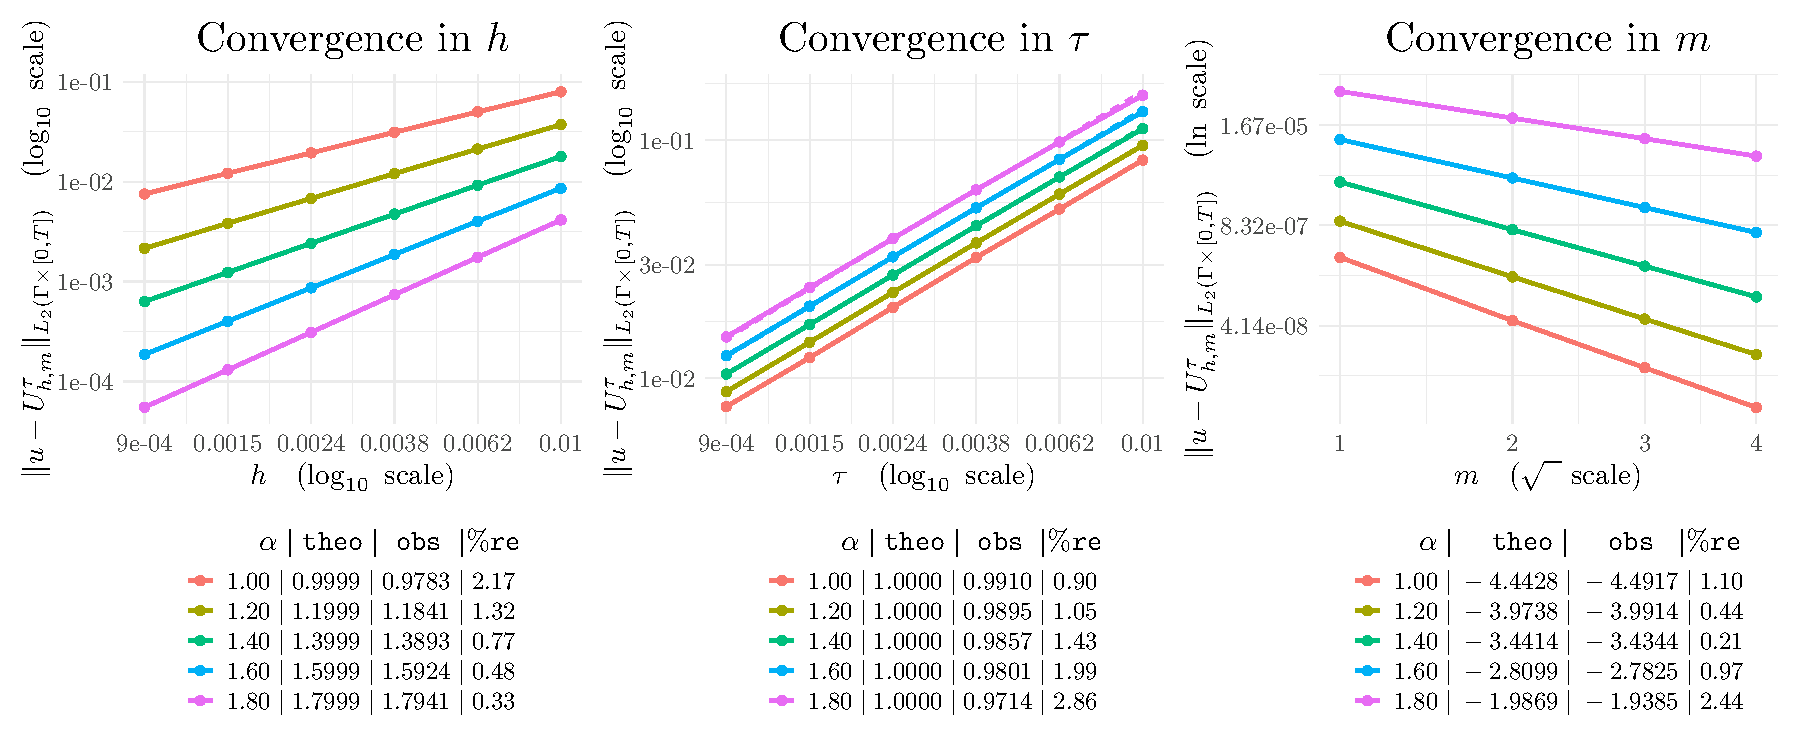
\includegraphics[width=0.99\textwidth]{Fig/p_all_nicer_tadpole_with_logtau_and_tauminustwo.pdf}
\caption{Comparison between the theoretical and observed convergence behavior of the $\|u-U_{h,m}^\tau\|_{L_2(0,T;L_2(\Gamma))}$-error with respect to $h$, $\tau$, and $m$. The left and center panels display the convergence with respect to $h$ and $\tau$, respectively, on a $\mathrm{log}_{10}$-$\mathrm{log}_{10}$ scale, while the right plot shows the exponential decay in $m$ on a semi-$\ln$ scale, with $m$ plotted on a square-root scale. Dashed lines indicate the theoretical rates, and solid lines represent the observed error curves. 
%The legends report the theoretical $(\mathtt{theo})$ and observed $(\mathtt{obs})$ values, namely, $\alpha-\epsilon$ and $s_h$ for the $h$-convergence study, $1$ and $s_\tau$ for the $\tau$-convergence study, and $-2\pi\sqrt{1-\sfrac{\alpha}{2}}$ and $s_m$ for the $m$-decay study. 
The legends report the value of $\alpha$, the theoretical $(\mathtt{theo})$ and observed $(\mathtt{obs})$ values, together with the relative percentage error $(\mathtt{\%re})=100|\mathtt{theo}-\mathtt{obs}|/|\mathtt{theo}|$. For the $h$-, $\tau$-, and $m$-studies, $(\mathtt{theo},\mathtt{obs})$ corresponds to $(\alpha-\epsilon,s_h)$, $(1,s_\tau)$, and $(-2\pi\sqrt{1-\sfrac{\alpha}{2}},s_m)$, respectively.}
\label{fig:combined_cov_rates}
\end{figure}

\section{Conclusions and Future Work}
\label{conclusion}
We have presented a comprehensive numerical framework for the approximation of fractional diffusion equations on compact metric graphs. By combining recent analytical developments for fractional operators on metric graphs with efficient numerical techniques, it establishes a foundation for the study and computation of nonlocal diffusion processes on network domains.

There are several natural extensions of this work for future investigation. First, the framework can be generalized to incorporate operators $L =\kappa^2 -\nabla\cdot(\mathbf{H}\nabla)$, where $\mathbf{H}$ is a symmetric and positive definite matrix. Second, our approach can be extended to fractional time derivatives, replacing the classical time derivative with a Caputo or Riemann–Liouville derivative. Inclusion of memory effects would improve modeling capabilities for anomalous diffusion processes \cite{Evangelista2018Fractional, Metzler2000Therandomwalksguide}. Third, building on  \cite{Glusa2021errorestimates}, a natural extension is the study of optimal control problems governed by space-time fractional models on metric graphs. Fourth, although we focused on metric graphs, the proposed spectral-rational framework relies only on the functional calculus of self-adjoint operators with compact resolvent. Consequently, it is expected to extend naturally to fractional diffusion problems on bounded Euclidean domains and compact Riemannian manifolds using standard finite element discretizations. Finally, replacing the right-hand side with a stochastic forcing term, particularly space-time white noise, would facilitate modeling stochastic fractional diffusion processes on graphs.



\section*{Acknowledgments}
The authors thank the anonymous reviewers for their valuable suggestions. This work is supported in part by funds from the National Science Foundation (NSF: \# 1636933 and \# 1920920).

\section*{Funding}
Funding information here.

\bibliographystyle{plain}
\bibliography{reference}


%USE THE BELOW OPTIONS IN CASE YOU NEED AUTHOR YEAR FORMAT.
%\bibliographystyle{abbrvnat}
%\bibliography{reference}


\end{document}
